\section{Evaluation}

\subsection{Configuration}

We conducted the extensive experiments to evaluate the performance of the methods proposed in this work. In the experiments, we use four nodes as the workers and one node as the master. Each node has two eight-core Xeon-2670 CPUs and 64GB memory. The file system is mounted on a SAS disk, running the RedHat Enterprise Linux 5 (kernel 2.6.18). The JDK version is 1.7.0 for Spark 1.6 and Spark Job Server 0.6.2. We record not only the execution time of each application, but also the detailed runtime situations.

\begin{table}[!t]
\small
\centering
\caption{Function APIs in each Application}
\begin{tabular}{ c | c | c | c }

\hline
\textbf{App} & \textbf{Stages} & \textbf{Function API(s)} & \textbf{Cache} \\
\hline
Grep & 1 & \textit{filter} & No \\
\hline
WC & 2 & \textit{flatMap} \& \textit{reduceByKey} & No \\
\hline
Sort & 3 & \textit{distinct} \& \textit{sortByKey} & No \\
\hline
PR & N & \textit{groupByKey} \& \textit{map} \& \textit{reduceByKey} & Yes \\
\hline

\hline
\end{tabular}
%\vspace{1mm} 
%\vspace{-8mm}
\label{table:app}
\end{table} 

We choose four typical benchmark applications in Spark to evaluate the performance: Grep, Sort, WordCount(WC) and PangeRank(PR). Grep has only one stage: it filters the records that do not satisfy the conditions. WC has two stages: it counts the number of each key in the input file. Sort has three stages: it sorts all records by key in the input file. While PR is a typical iterative computations, one of its most important features is that it will cache the data in memory. We choose these four benchmarks because these applications contain different function APIs, as shown in Table~\ref{table:app}. For Sort and WC, the datasets are produced by HiBench Random Writer with 1B unique key numbers. The sizes of the input datasets for Sort and WC are 30GB and 50GB, respectively. For Grep and PR, we use the real graphs, webbase-2001 (30GB)~\cite{boldi:webgraph}, to evaluate the performance of MURS. The key-value pairs of each record in all input dataset have the similar size. We use the heap size to evaluate different memory pressure. The garbage collection time is used to measure the memory pressure. These applications are grouped to evaluate different scenes and submitted to the Spark Job Server together.

\subsection{Memory pressure without caching}

Most current data processing systems are designed based on MapReduce. But only a part of them provide the in-memory computing model that caches the data in memory to speed up the system. Thus, we first evaluate these applications without caching the data in memory, which represents the common frameworks that work with the key-value pairs, such as Hadoop and Hive.

We choose three applications: Sort, WC, and Grep. These applications do not perform the caching operations. Each application has similar implementation in MapReduce. Grep reads the data from the disk and filters these records which satisfy the given conditions. Most data objects are temporary. The shuffle buffers in Sort and WC contain the data objects with long lifetime. Thus the tasks in Sort and WC are the light to heavy tasks in MURS. The results of each submission are shown in Figure~\ref{fig:pressurewithoutcache}. The best improvement achieved by MURS is 1.8x to 2.9x compared to Spark in each evaluation. The reduction of the garbage collection contributes most to the improvement.

\begin{figure*}[!t]
\centering
\subfigure[Sort+Grep]{
\label{fig:subfig:sort-grep}
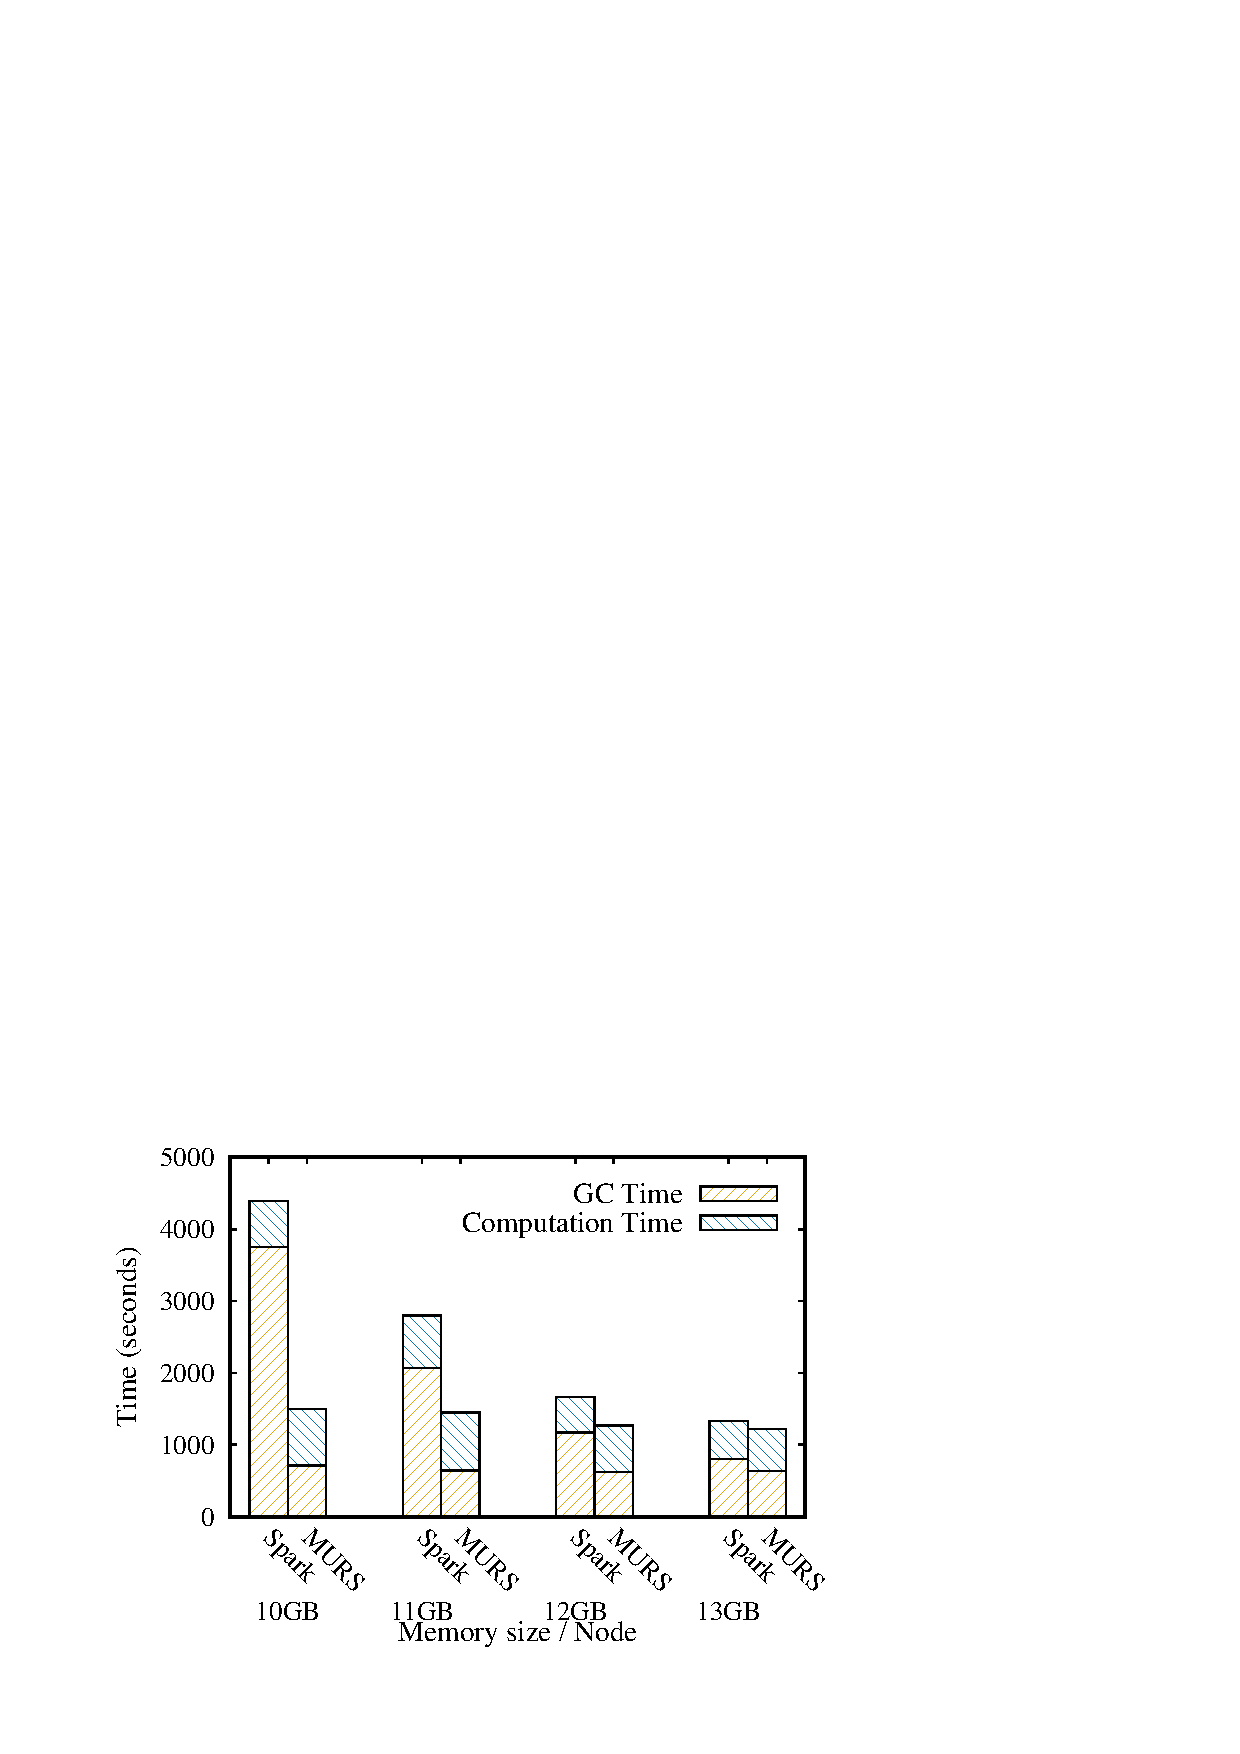
\includegraphics[width=0.3\textwidth]{sort-grep.pdf}}
%\hspace{-3ex}
\subfigure[WC+Grep]{
\label{fig:subfig:wc-grep}
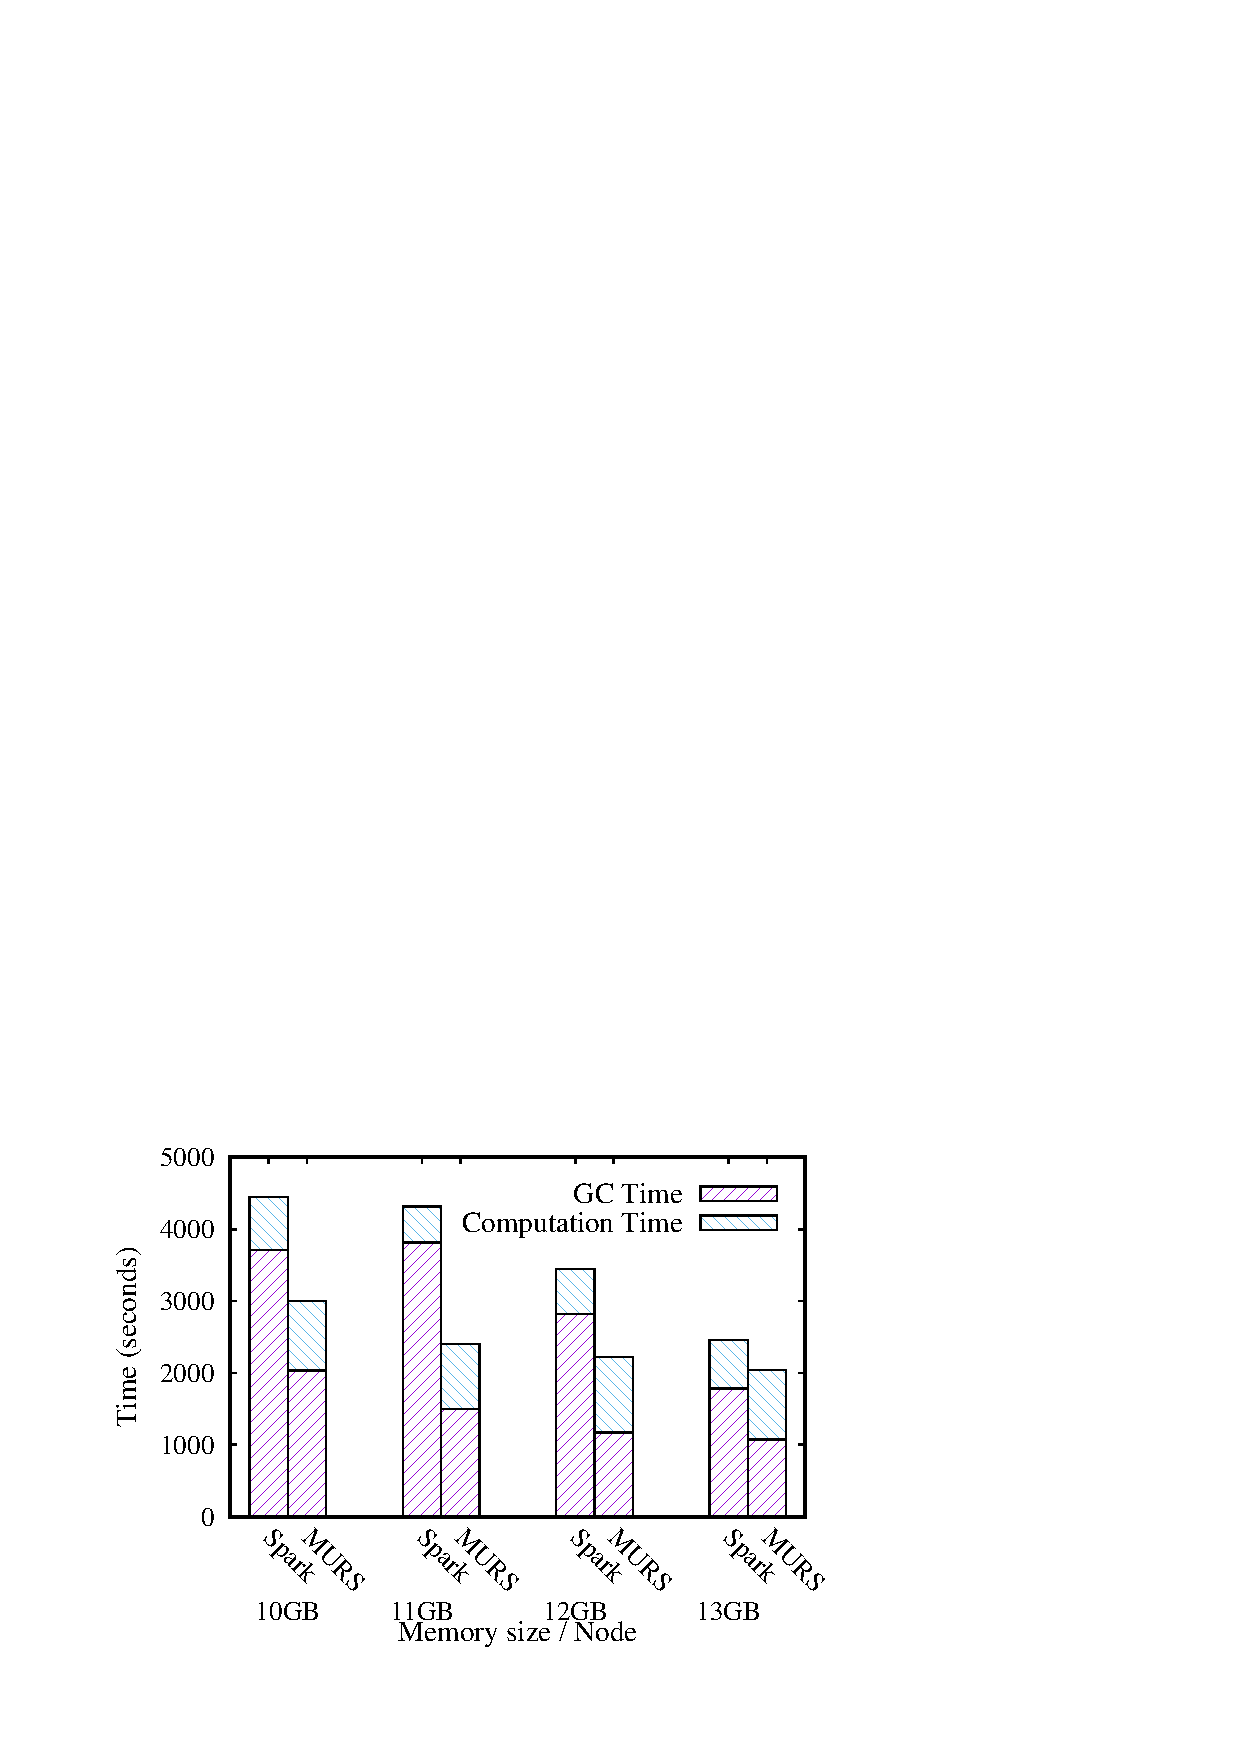
\includegraphics[width=0.3\textwidth]{wc-grep.pdf}}
%\hspace{-1.9ex}
\subfigure[Sort+WC+Grep]{
\label{fig:subfig:sort-wc-grep}
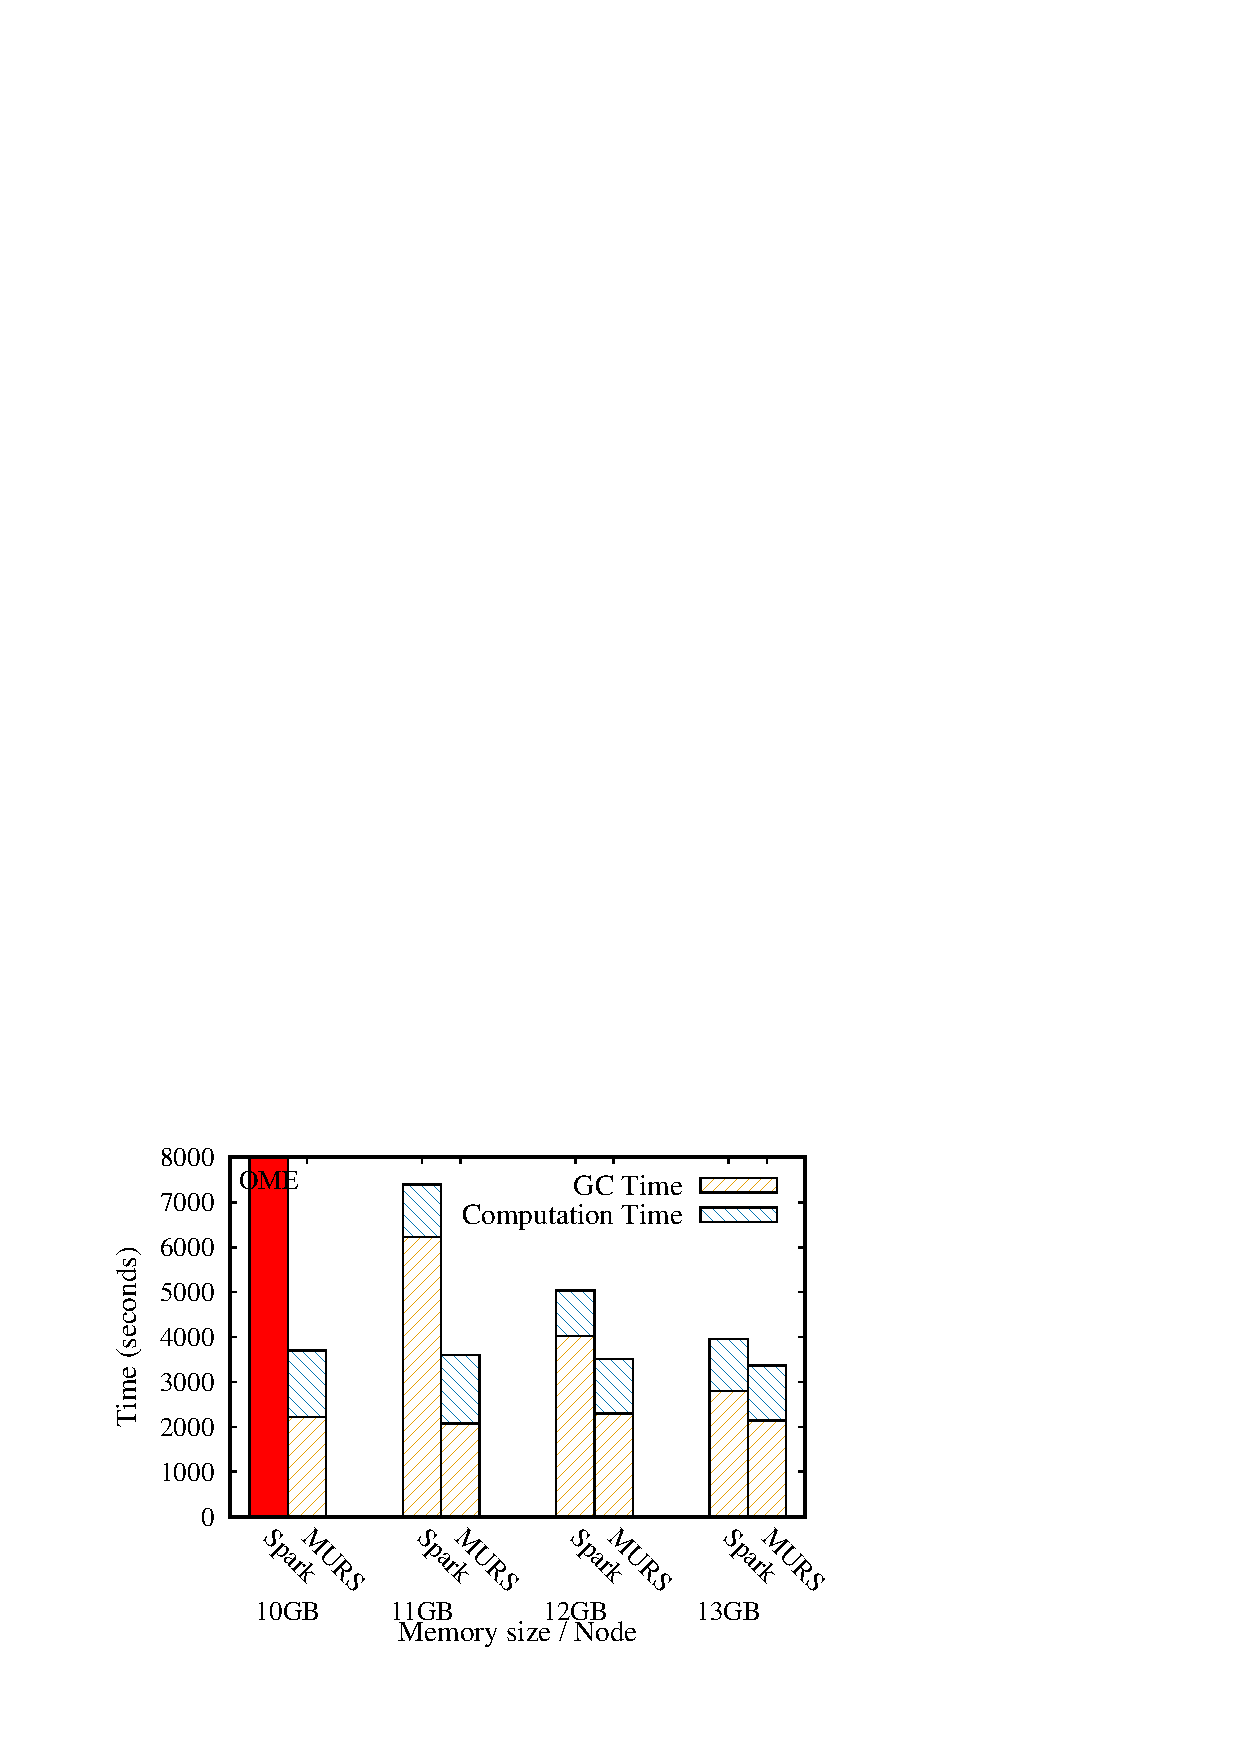
\includegraphics[width=0.3\textwidth]{sort-wc-grep.pdf}}
%\hspace{-1.9ex}
%\subfigure[Active tasks]{
%\label{fig:subfig:activetasks}
%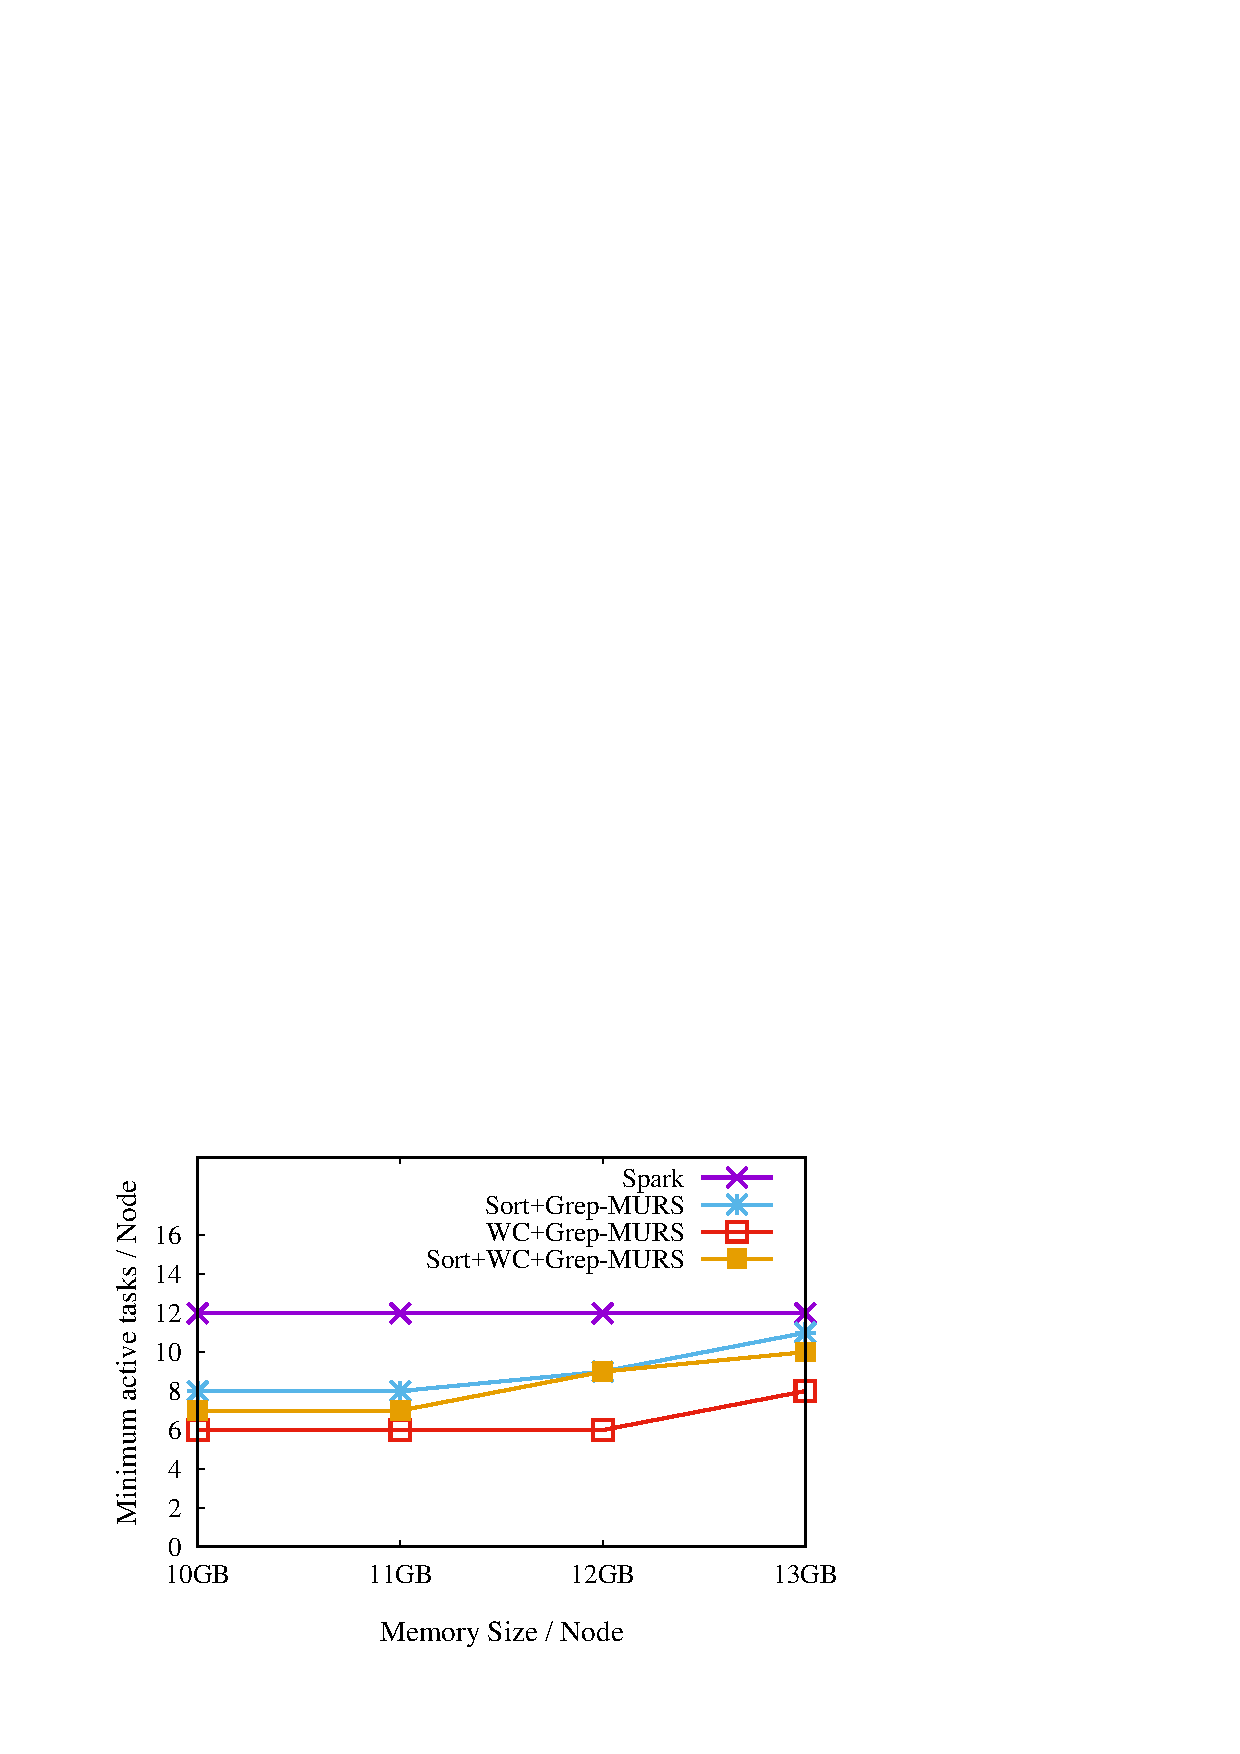
\includegraphics[width=0.3\textwidth]{active-task.pdf}}
%\vspace*{-5mm}
\caption{Results of memory pressure without caching}
%\vspace*{-4mm}
\label{fig:pressurewithoutcache}
\end{figure*}

When two applications are submitted to the server, MURS works better in Sort and Grep. Comparing Sort to WC, the heavy memory pressure occurs in the different phase. The \textit{sort} operation is implemented in the \textit{read phase} of the tasks. Thus the tasks in the last stage of Sort suffer from the heavy memory pressure during their read phases. However, the \textit{reduce} operation in WC is realized in the \textit{write phase} of the tasks. The heavy memory pressure is caused by the write phase of the tasks in the first stage. Moreover, massive temporary data objects are produced by the function API \textit{flatMap} before the write phase. They may be currently alive in the heap during the write phase in WC. Although the tasks in Sort belong to the linear memory usage model and the tasks in WC are sub-linear, MURS suspends more tasks in WC as the heap size in WC is occupied by the temporary data objects, as shown in Figure~\ref{fig:active-task}. These temporary data objects result in frequenter garbage collections. We can see that suspension in MURS is determined not only by the memory usage models, but also by the current usage of the heap. 

When three applications are submitted, out-of-memory (OME) is thrown by the server. Although the live shuffle buffer in this case is smaller than the case with two applications, some other data objects occupy much heap space, such as the recording of living applications, the handler of disk writing, and the global configurations of Spark. Spark provides the spilling capability to overcome the shortage of memory. However, it cannot completely avoid the OME.

MURS mitigates the memory pressure in each application and we find that the performance slows down tardily along with the heap size. The result shows that the cost of garbage collection is stable. As MURS suspends the heavy tasks, the slow increase in execution time due to the increase in computation time.  

\begin{figure}[!t]
\centering
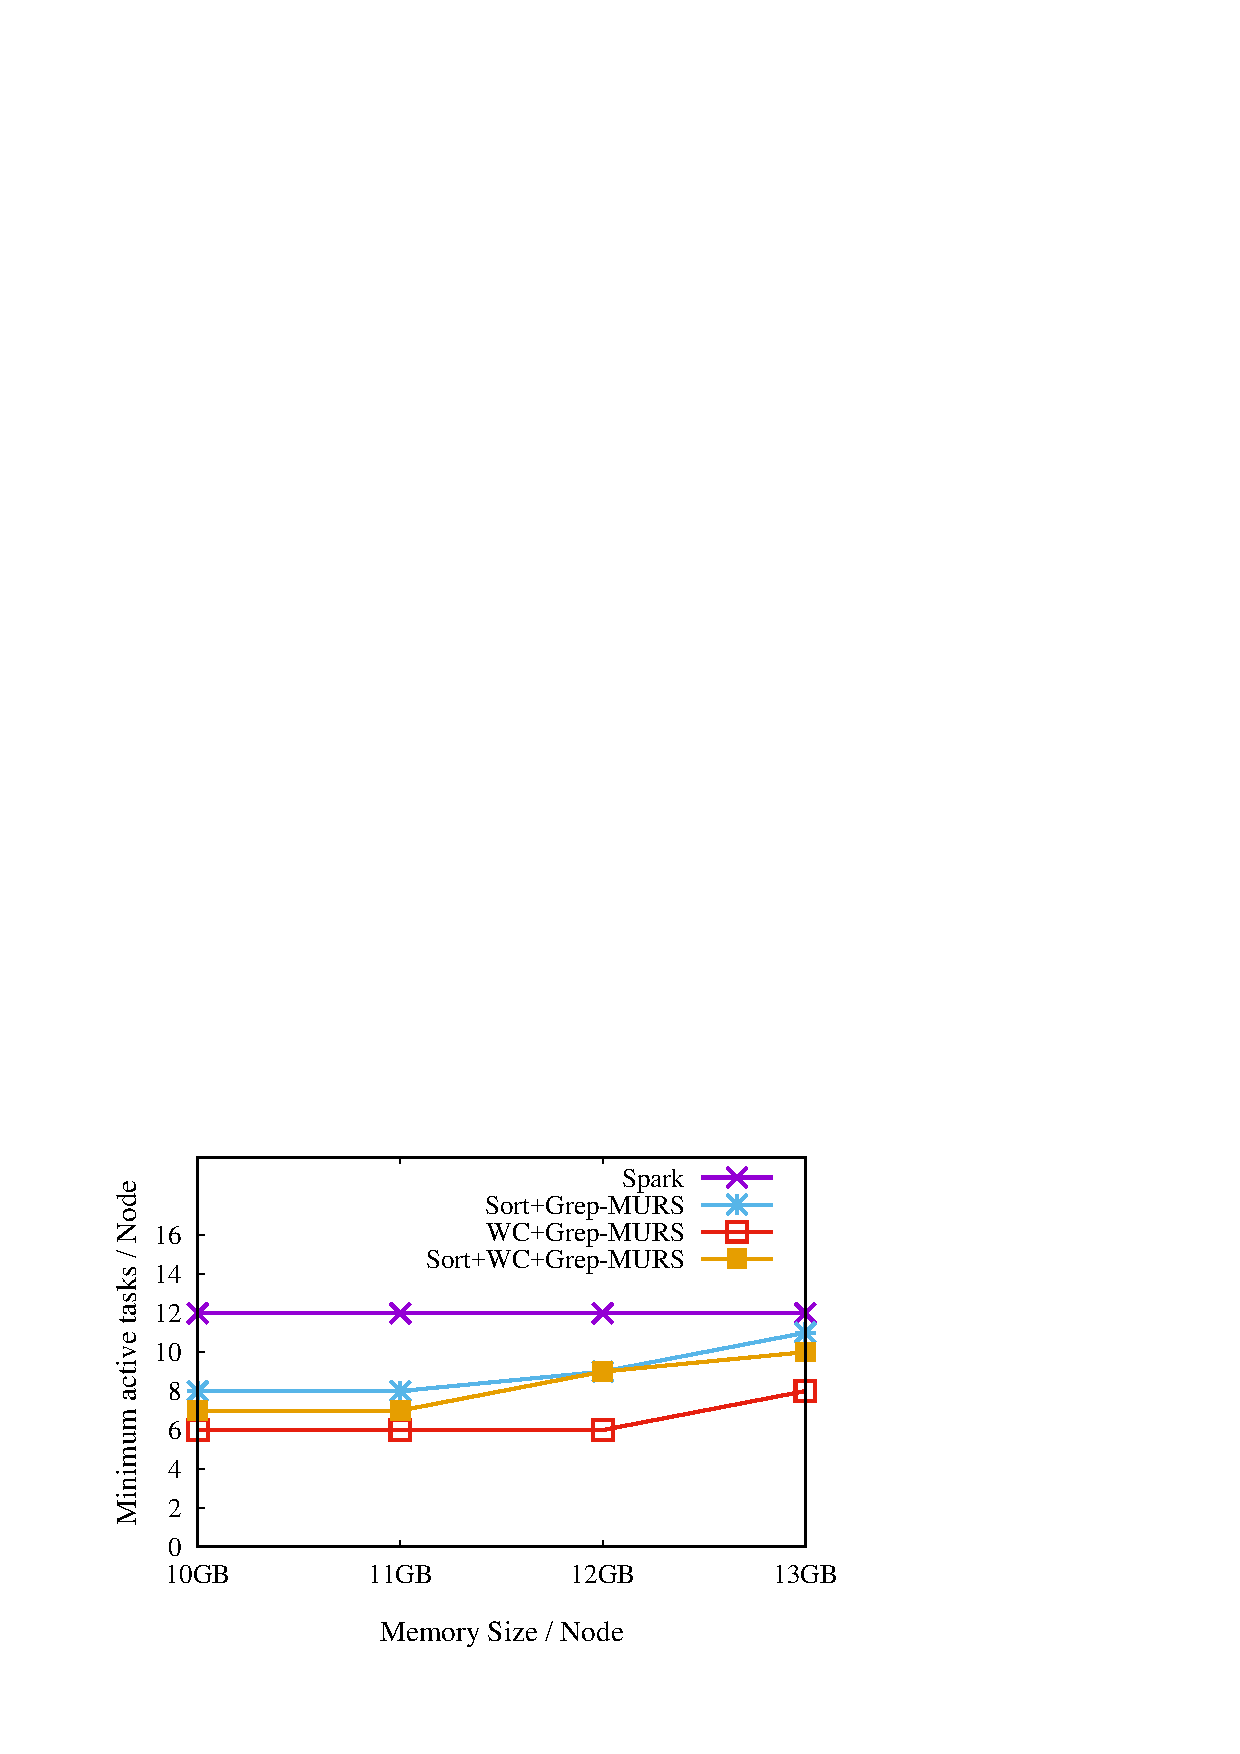
\includegraphics[width=0.35\textwidth]{active-task.pdf}
%\vspace{-2mm}
\caption{The minimum active tasks in each server}
%\vspace{-4mm}
\label{fig:active-task}
\end{figure}

\subsection{Memory pressure with caching}

Some frameworks provide the caching mechanism for in-memory computation, such as Spark and Flink. Although the in-memory data caching speeds up the execution of a job, some works~\cite{bu:bloat, nguyen2015facade} show that it results in greater memory pressure because the cached data live as long as the job. Tracing these data is expensive. Also, the memory pressure means that there is less accessible memory space for the job execution.


PR and WC are used as the experimental applications. PR is an iterative application. In the experiments, we run 5 iterations of the application. PR caches the intermediate data in memory after the first iteration. WC is submitted at the second iteration. We adjust the heap size to show the performance of MURS, while the input dataset is 30GB, as shown in Figure~\ref{fig:cache-total}. When the heap size is less than 17GB, the server version of Spark throws the Out-of-Memory error (OME). MURS can provide the service when the heap size is reduced to 15GB. While they are both working, MURS improves the performance by up to 23.4\%, and the memory pressure is reduced by 65.4\%.

\begin{figure}[!t]
\centering
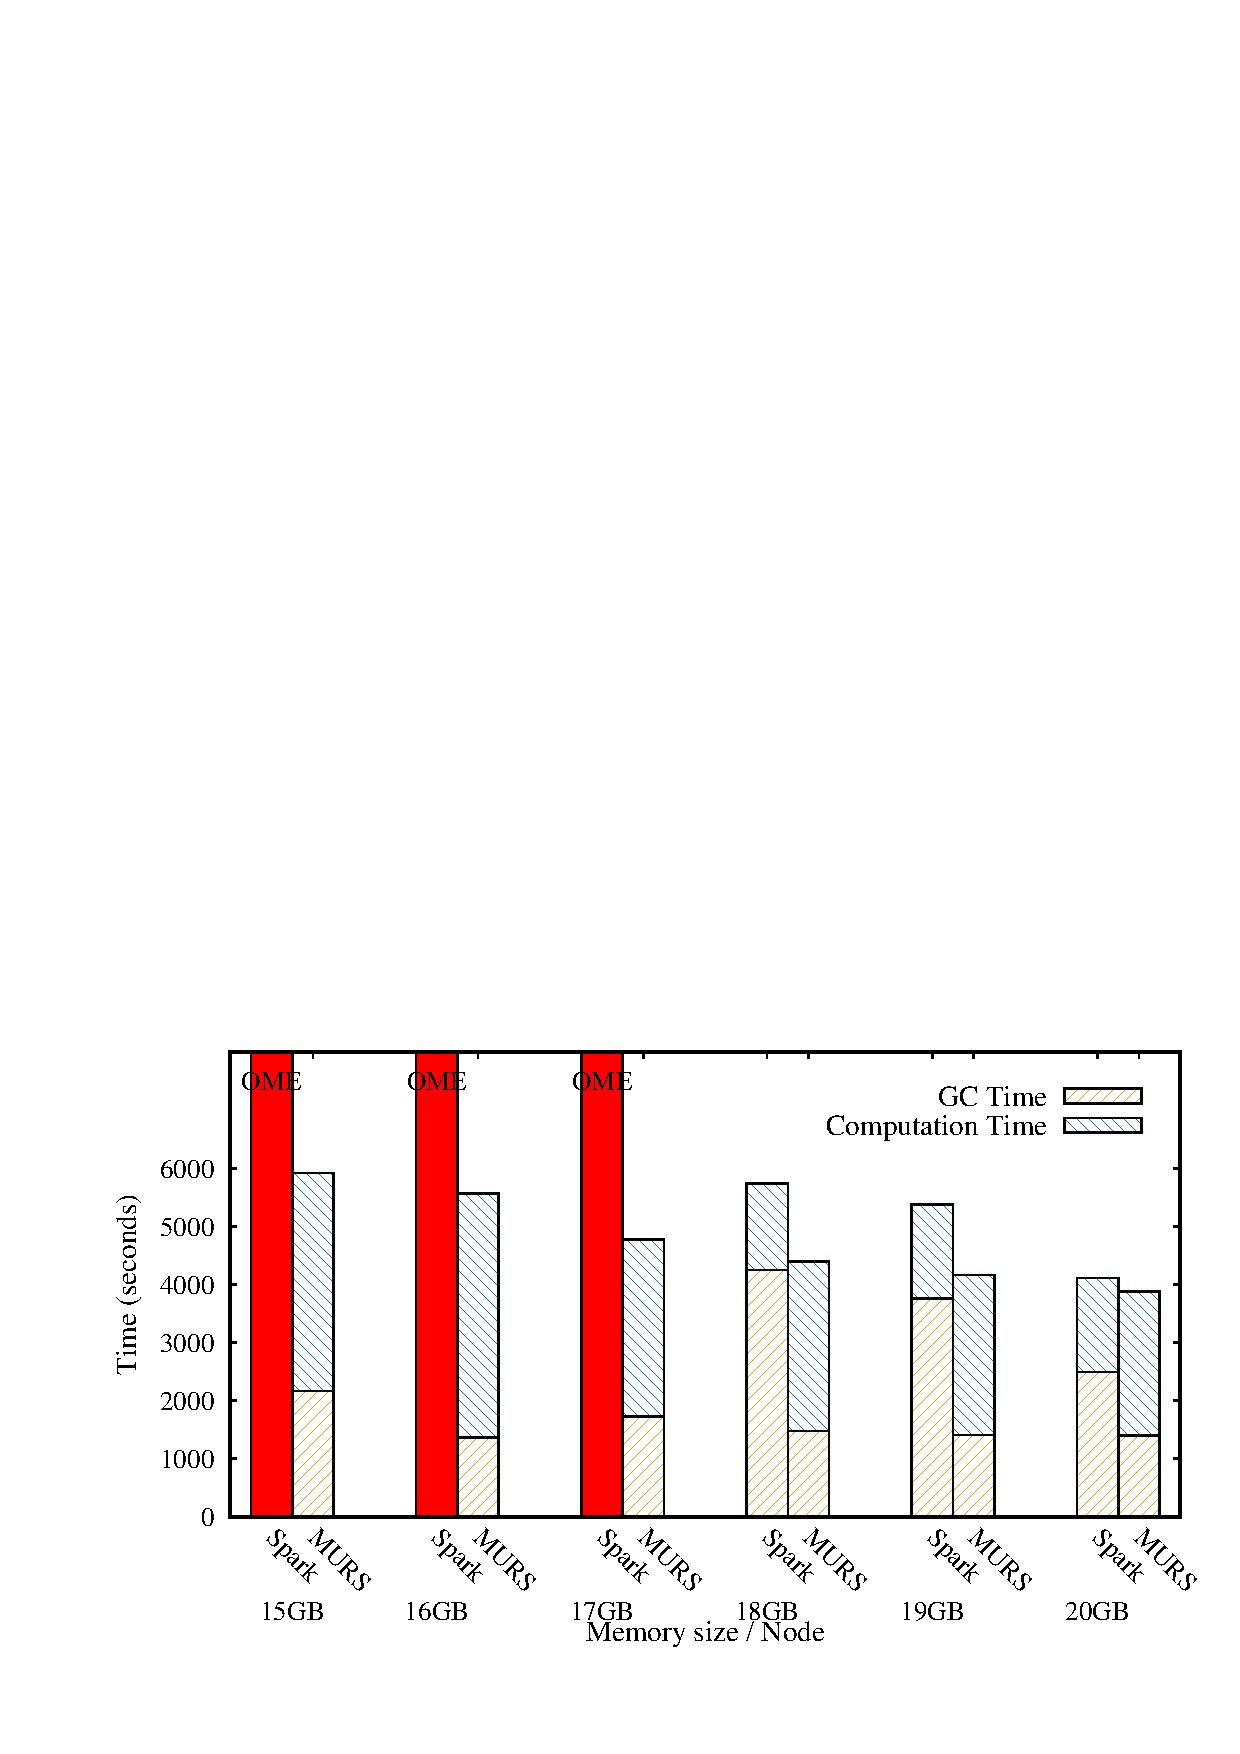
\includegraphics[width=0.45\textwidth]{cache-total.pdf}
%\vspace{-2mm}
\caption{The Execution and GC Time of PR and WC in Server}
%\vspace{-4mm}
\label{fig:cache-total}
\end{figure}

Less heap size in each node means more memory pressure in the server. When the heap is exhausted, tasks will throw the OME. With the caching data in memory, The server version of Spark throws the OME as the heap size of each node is 17GB. However, MURS is able to mitigate the heavy memory pressure and still performs well when the heap size of each node is reduced to 15GB. MURS suspends heavy tasks and  thus the remaining light tasks can utilize more memory. Figure~\ref{fig:cache-peak} shows that the peak memory usage of all tasks in MURS is consistently larger than that in Spark. The number of active tasks in MURS is reduced to ensure there is the memory available for the running tasks. In other words, MURS has better scalability than the server version of Spark.

\begin{figure}[!t]
\centering
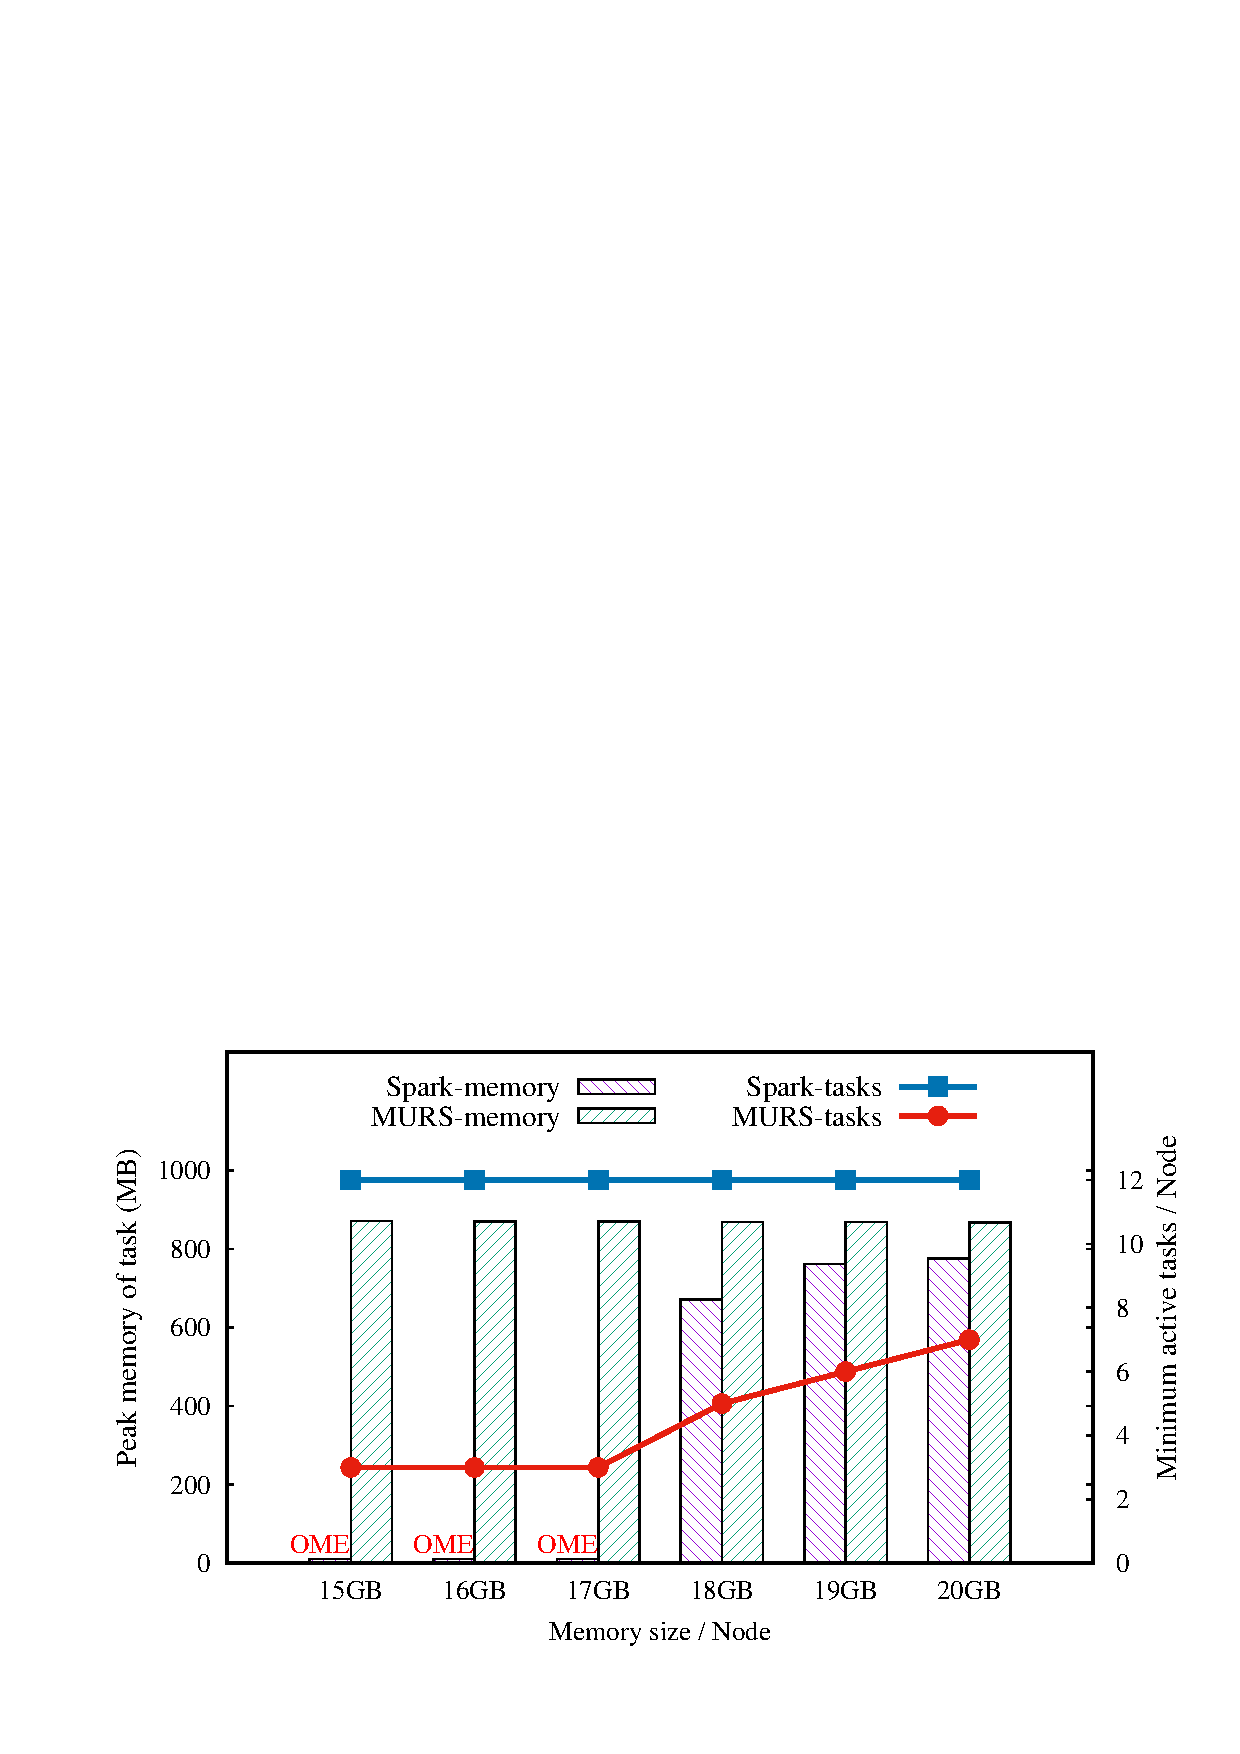
\includegraphics[width=0.45\textwidth]{cache-peak.pdf}
%\vspace{-2mm}
\caption{The peak usage memory of tasks and minimum active tasks}
%\vspace{-4mm}
\label{fig:cache-peak}
\end{figure}

\subsection{Potential starvation in MURS}

The mitigation strategy of memory pressure delays the computation of suspended tasks. This may cause the starvation of the suspended tasks. MURS address this issue in the application level. 

The settings of the experiment presented in this subsection are the same as those in the previous subsection. When PR and WC are submitted to the server, the tasks of PR have the same \textit{write phase} as the tasks of WC, but contain more function APIs. Thus the tasks of PR are mostly classified as the heavy tasks. They will be suspended when the memory pressure is heavy. The execution time of each application is shown in Figure~\ref{fig:cache-prwc}. The result shows there is no starvation for PR. Benefiting from MURS, the performance of PR is improved by up to 24.4\%. The performance of WC, which contains light tasks, also achieves a 29.8\% improvement. 

\begin{figure}[!t]
\centering
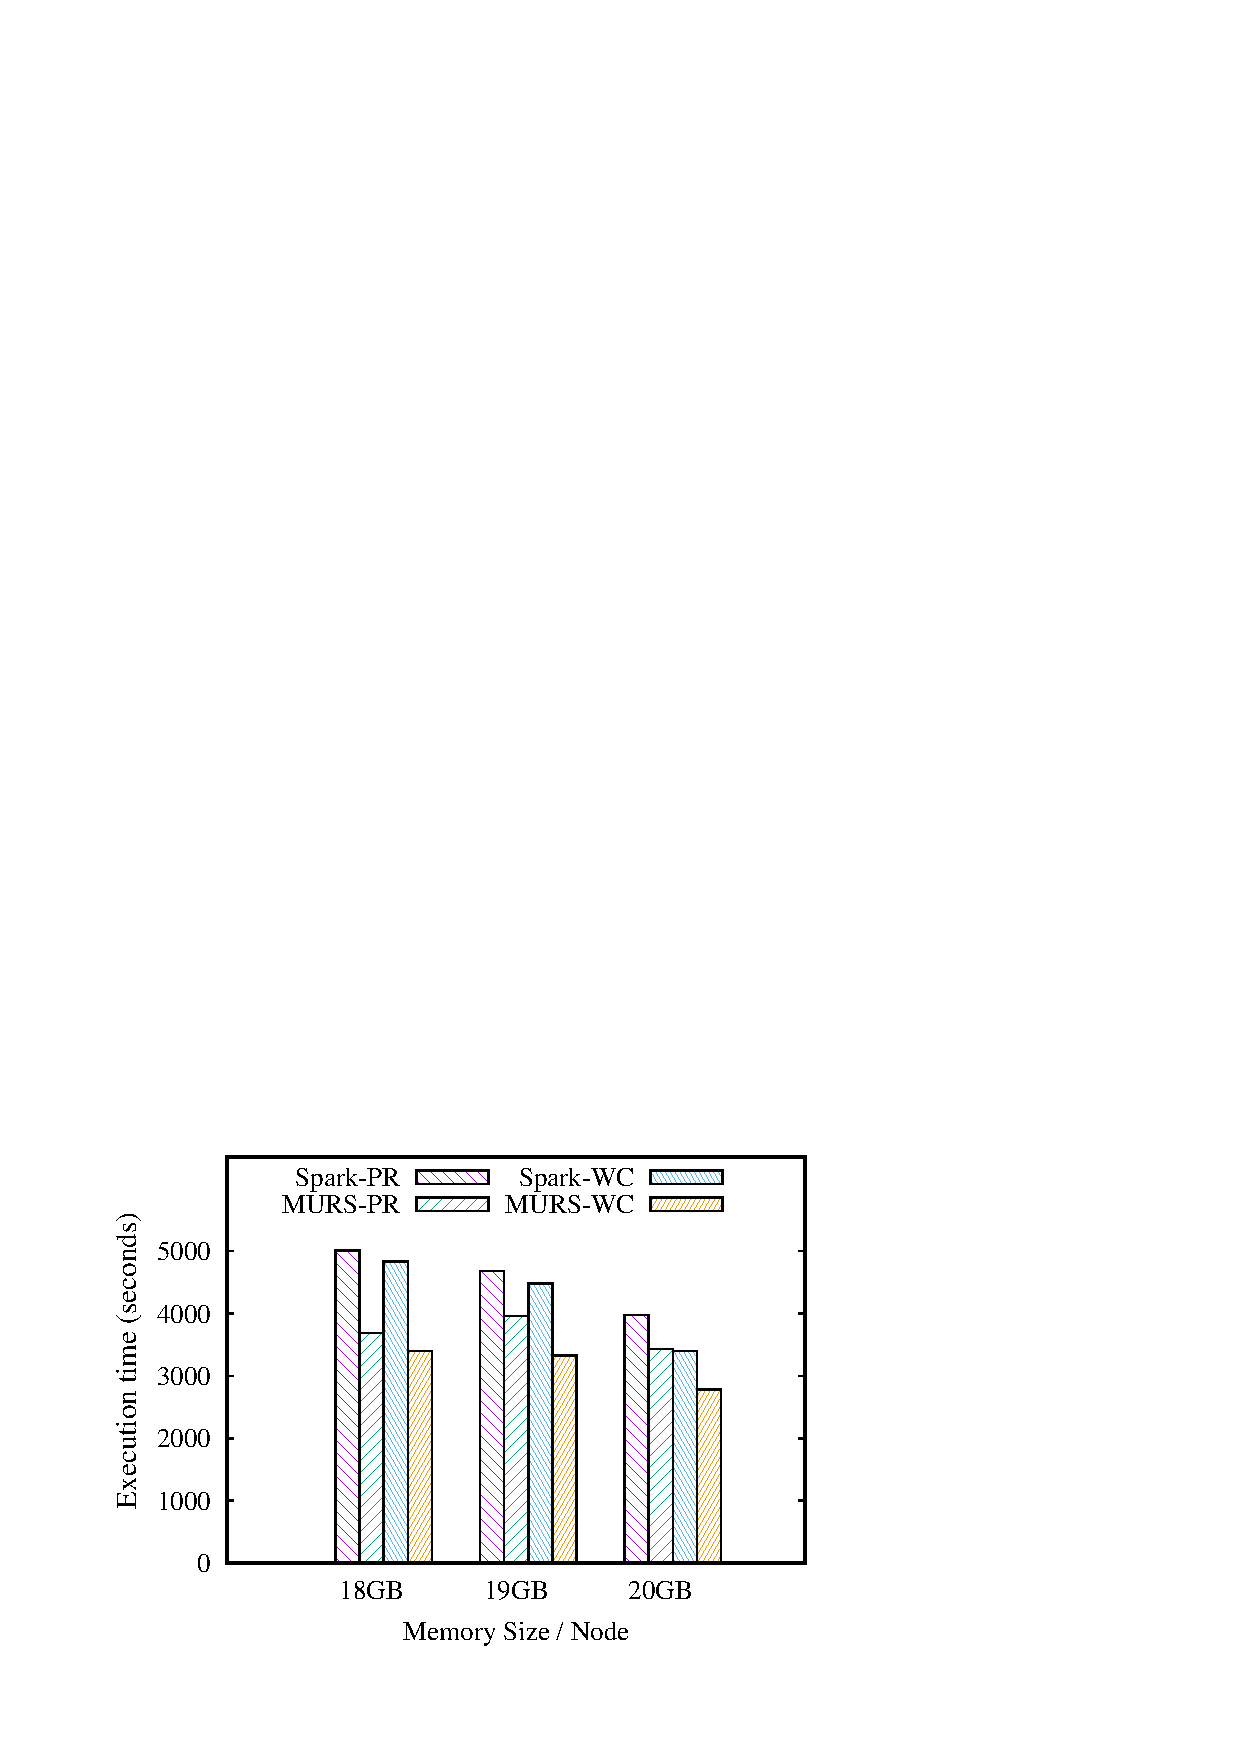
\includegraphics[width=0.35\textwidth]{cache-prwc.pdf}
%\vspace{-2mm}
\caption{The execution time of each application}
%\vspace{-4mm}
\label{fig:cache-prwc}
\end{figure}

MURS applies the FIFO algorithm when it resumes the suspended tasks. This avoids the long wait of these tasks. Otherwise, suspending these tasks is going to mitigate the memory pressure not only for the currently running light tasks, but also the heavy tasks running next. In the application level, the transient suspension and light memory pressure are actually the trade-off made by MURS. 

\subsection{Avoiding the spill}

MURS sets the alarming threshold to avoid the spill when the memory pressure is heavy in the systems that allow the spill. In the experiments presented in last subsection, we also measure the spilling tasks. MURS estimates the size of the required memory space for each task, and ensures that the running tasks can complete with the remaining memory space. As the estimation is inaccurate to some extent, we find that fewer tasks will spill in MURS, as shown in Table~\ref{table:spill}. There are no the spill tasks in WC in MURS, while the spill tasks in PR decrease from 32\% to 2.5\%.

\begin{table}[!t]
\small
\centering
\caption{Spill Tasks in MURS and Spark}
\begin{tabular}{ c | c | c | c | c | c | c | c }

\hline
\multirow{2}{*}{} & \multirow{2}{*}{\textbf{App}} & \multicolumn{3}{| c |}{\textbf{Spill Percentage}} & \multicolumn{3}{| c }{\textbf{Spill Size (MB)}} \\
\cline{3-8}
 & & total & spill & percent & min & mid & max \\
\hline
\multirow{2}{*}{Spark} & WC & 1000 & 91 & 9\% & 0 & 0 & 710 \\
\cline{2-8}
 & PR & 1500 & 480 & 32\% & 310 & 367 & 439 \\
\hline
\multirow{2}{*}{MURS} & WC & 1000 & 0 & 0\% & - & - & -  \\
\cline{2-8}
 & PR & 1500 & 37 & 2.5\% & 0 & 0 & 458 \\
\hline

\hline
\end{tabular}
%\vspace{-2mm}
 
%\vspace{-6mm}
\label{table:spill}
\end{table}

We notice that the error exists when avoiding the spill. The sampler in MURS counts two important metrics for a task: the percentage of the processed records in the total records, and the currently allocated memory space for this task. We can quickly obtain the required memory space based on these two metrics. When the memory pressure reaches the alarming threshold, we suspend a part of the running tasks and leave enough memory space for the remaining running tasks. As the estimate is based on sampling, the error exists in terms of the estimated size of the allocated memory space, especially when the value in some key-value pairs is a collection. Different records have different sizes because the number of values inside a collection is different, such as \textit{groupByKey} in PR. Some hot keys may result in a substantial error. Thus, there are even fewer spilling tasks in MURS that the figures reported in the experiments.

















\begin{comment}

\subsection{Configuration}

We use four nodes as workers and one node as the master in the experiments. Each node has two eight-core Xeon-2670 CPUs and 64GB memory. The file system is mount on one SAS disk, running RedHat Enterprise Linux 5 (kernel 2.6.18). The JDK version is 1.7.0 for Spark 1.6 and Spark Job Server 0.6.2. We count not only the execution time of each application, but also the details of all tasks. Some important configurations are set to be the same in both MURS and Spark, as shown in Table~\ref{table:config}. The memory of each executor is set to be 15GB.

\begin{table}[!t]
\small
\centering
\caption{Important Configurations in MURS and Spark}
\begin{tabular}{ c | c | c }

\hline
\textbf{Configurations} & \textbf{Default} & \textbf{Value} \\
\hline
spark.serializer & No & KryoSerializer \\
\hline
spark.cores.max & No & 48 \\
\hline
spark.shuffle.compress & Yes & true \\
\hline
spark.shuffle.manager & Yes & sort \\
\hline
spark.memory.fraction & Yes & 0.75 \\
\hline
spark.memory.storageFraction & Yes & 0.5 \\
\hline

\hline
\end{tabular}
%\vspace{-2mm} 
%\vspace{-6mm}
\label{table:config}
\end{table} 

We choose four typical benchmark applications in Spark to evaluate the performance: Grep, Sort, WordCount(WC), and PangeRank(PR). Grep has only one stage: it filters the records that do not satisfy the conditions. WC has two stages: it counts the number of each key in the input file.  Sort has three stages: it sorts all records by key in the input file. While PR is a typical iterative computations, and one of its most important features is that it will cache data in memory. We choose these four benchmarks because these applications contains all three models. We will show the details later. For Grep, Sort, and WC, the datasets are produced by HiBench Random Writer with different unique key numbers (1M and 1B), both with the size of 50GB. And for PR, we use the real graphs: webbase-2001 (30GB)~\cite{boldi:webgraph} to evaluate the performance of MURS. Key-value pairs of each record in all input dataset have the similar size, thus we can simply analyze the memory usage model by function API. These applications are grouped to evaluate different scenes and submitted to Spark Job Server together.

\subsection{Memory pressure without caching}

Most current data processing systems are designed based on MapReduce, but only parts of them provide the in-memory computing model that caches data in memory to speed up the system. Thus, we first evaluate these applications without caching data in memory to stand for common frameworks working with key-value pairs, such as Hadoop and Hive.

We choose Grep, Sort, and WC to form the benchmark set. The function APIs in each job are shown in Table~\ref{table:grep-sort-wc}. Grep has no shuffle operation. WC and Sort jobs are split by the shuffle operations. Tasks in the first stage of WC result in more memory pressure than second stage, because most records are aggregated in the write phase. In contrast, Sort actually sorts keys in the read phase of tasks in the third stage. Jobs are simultaneously submitted to Spark Job Server. The execution time of each job is decreased by 20\% to 30\%. We count the execution time and garbage collection time of all tasks in each stage, as shown in Figure~\ref{fig:grep-sort-wc-gc}. Tasks with constant model (Stage 2-3) all have a short execution time. They also benefit from MURS and the execution time is decreased by 59\%, although the garbage collection time of them has less degradation. Execution time of tasks with sub-linear model (Stage 0) is decreased by 54\% and the reduction comes all from the mitigation of garbage collection. Execution time of tasks with linear model (Stage 5) is reduced by 50\%, and the garbage collection time is decreased by 58\%.

\begin{table}[!t]
\small
\centering
\caption{Function APIs in each Application without caching}
\begin{tabular}{ c | c | c | c }

\hline
\textbf{Application} & \textbf{Stage ID} & \textbf{Function API} & \textbf{Model}\\
\hline
\multirow{2}{*}{WC} & Stage 0 & \textit{reduceByKey} & sub-linear  \\
\cline{2-4}
 & Stage 1 & \textit{reduceByKey} & sub-linear \\
\hline
Grep & Stage 2 & \textit{filter} & constant \\
\hline
\multirow{3}{*}{Sort} & Stage 3 & \textit{flatMap} & constant \\
\cline{2-4}
 & Stage 4 & \textit{sortByKey} & linear \\
\cline{2-4}
 & Stage 5 & \textit{sortByKey} & linear \\
\hline

\hline
\end{tabular}
%\vspace{1mm} 
%\vspace{-8mm}
\label{table:grep-sort-wc}
\end{table}

%We chose Grep, Sort, and WC to group the submitted jobs. The function API in Grep is \textit{filter}, which does not distinguish the key and process each record. It just judges whether the record satisfies given conditions and writes it to disk; thus, all data objects are temporary data objects and the model belongs to the constant model. The function API in Sort is \textit{sortByKey}, which must shuffle all records and partition the records in order by key. Each record will be saved in shuffle buffer before writing to disk, thus it belongs to the linear model. The function API in WC is \textit{reduceBykey}, which distinguishes the key and aggregates the value. It is a typical sub-linear model. From the model, we find that tasks in Sort may have more impact on memory pressure. The result shows that the execution time of WC is decreased by 20\%, Grep is decreased by 15\%, and Sort is decreased by 13\%. We take the execution time and garbage collection time of tasks to analyze the improvement, as shown in Figure~\ref{fig:grep-sort-wc-gc}.

\begin{figure}[!t]
\centering
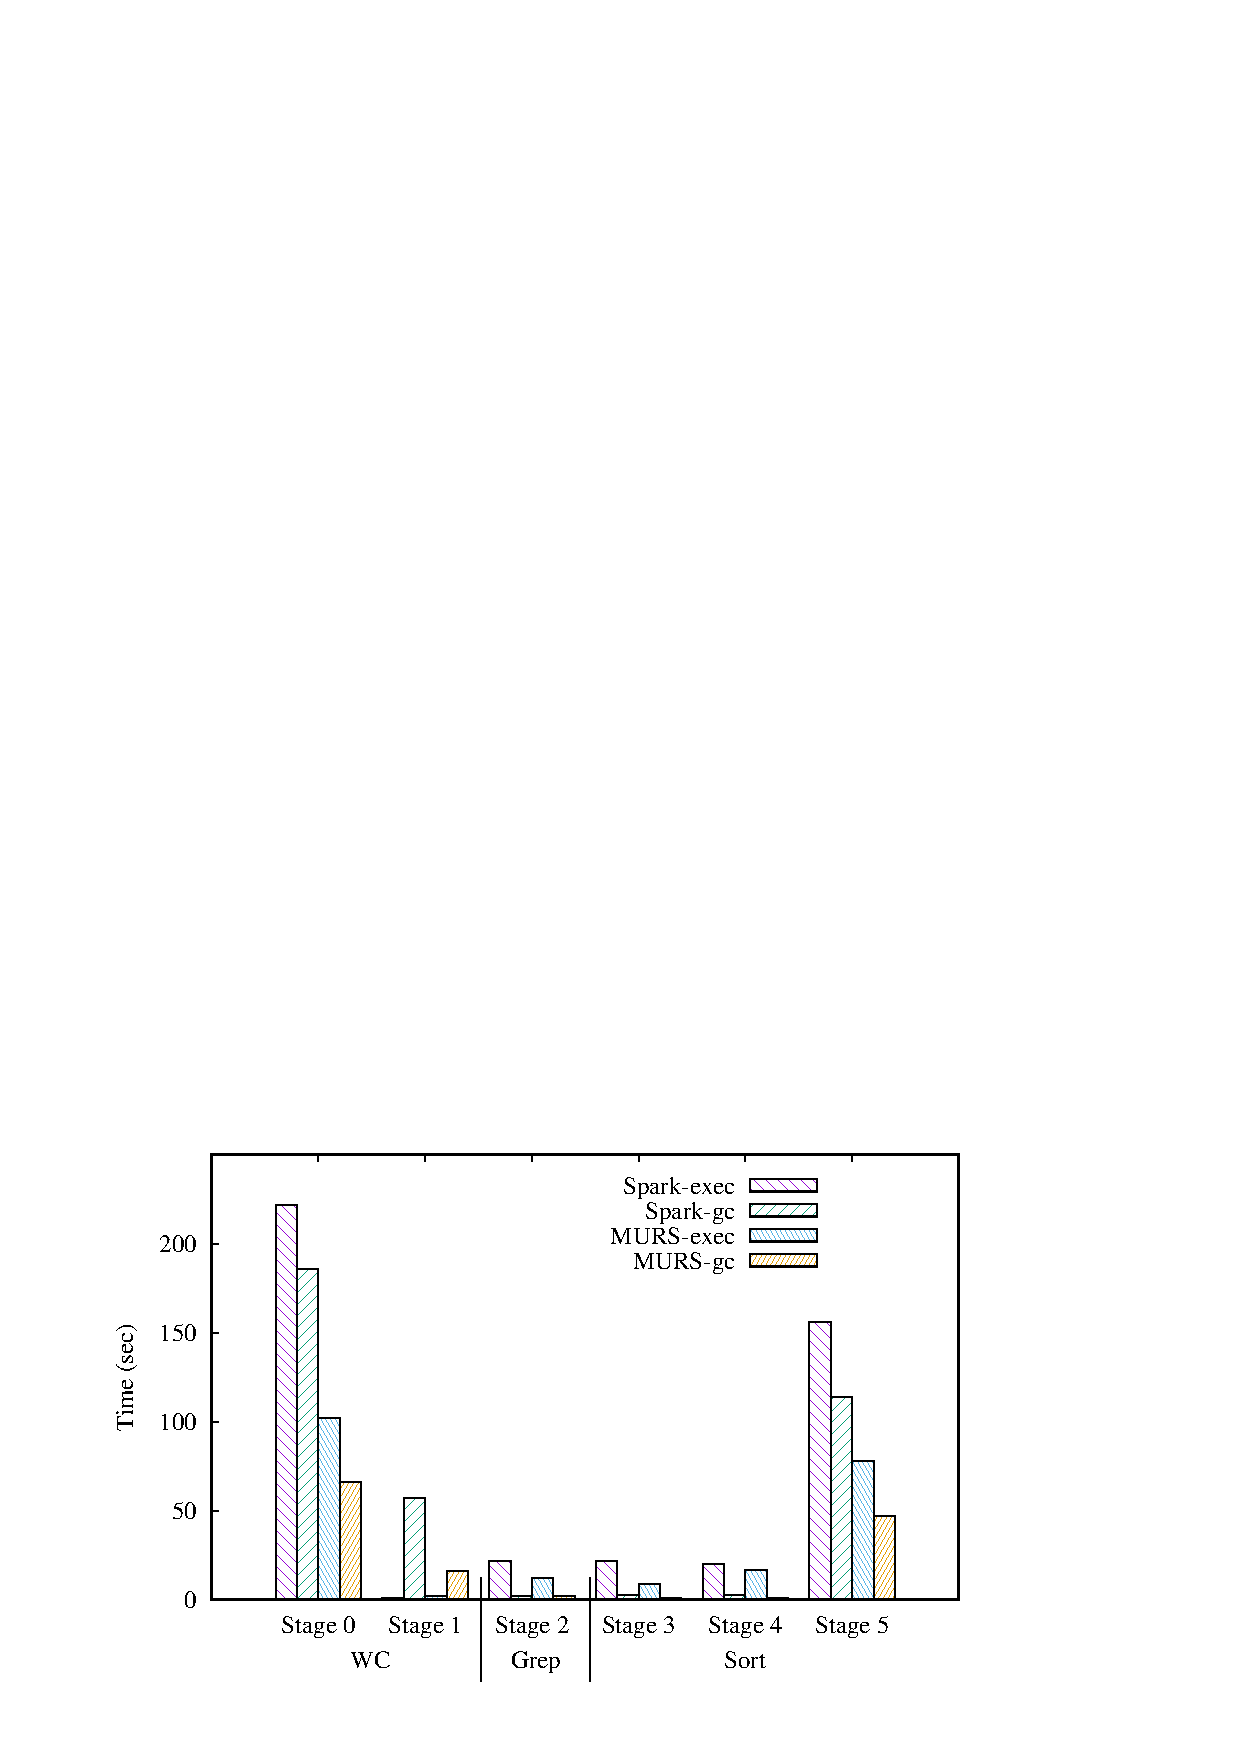
\includegraphics[width=0.4\textwidth]{grep-sort-wc-gc.pdf}
%\vspace{-2mm}
\caption{The Execution and GC Time of Tasks in Sort, Grep and WC}
%\vspace{-4mm}
\label{fig:grep-sort-wc-gc}
\end{figure}

Tasks with constant model in Stage 2 and Stage 3, along with tasks with sub-linear model in Stage 1, all benefit from MURS although the memory pressure is light. This is due to the parallelism in writing to disk, as Spark writes intermediate data in shuffle write phase to disk for checkpoint. Note that when these tasks are running, tasks in Stage 5 have not been launched. MURS is triggered when the proportion of used heap first touch the yellow value, it suspends some tasks in WC and decreases the parallelism in writing to disk. With enough bandwidth of writing to disk, these tasks still execute fast. We find that tasks in Stage 4 benefit less from the parallelism in writing to disk, because they are linear models and suspended by MURS when the proportion of used heap touches the yellow value. 

The reductions of Stage 0 and Stage 5 prove the mitigation on memory pressure through MURS. The garbage collection time in WC has a greater degradation than Sort. While WC suffers heavy memory pressure produced by Sort in Spark, MURS suspends tasks with linear models in Sort and ensures enough memory space for WC. Almost all reduction time comes from the mitigated memory pressure because there are no suspended tasks in WC. Sort gets more memory space after WC completes, and has less memory pressure than Spark. 

%As the Sort application is split into three stages, only tasks in the second stage (this stage just prepares records for the next stage and writes records to disk) and the third stage (this is the actual stage that sorts the key) is the linear model. The function API in the first stage is \textit{flatMap}, which flats the result and provides an iterator, thus it belongs to the constant model. We find that these tasks with sub-linear and linear models suffer greater memory pressure, and all benefit from MURS. However, we can see that the constant model is also a little better, although the garbage collection time has a lower percentage in the original execution time—such as tasks in Grep and the first stage of Sort. This is due to the parallelism in writing to disk. As other tasks suffer heavy memory pressure, MURS stops some tasks and prevents them from writing shuffle data to disk. The accessibility of the disk can be faster, and those running tasks with the constant model can quickly complete their operation on disk. 

\subsection{Memory pressure with caching}

Some frameworks provide caching mechanism for in-memory computation, such as Spark and Flink. Although the in-memory caching data speed up the execution of a job, some works~\cite{bu:bloat, nguyen2015facade} show that it results in greater memory pressure because the caching data live along with the job. Tracing these data is expensive and there is less accessible memory space for execution.

PR is an example of iterative computations that caches important intermediate data in memory. The function API in the first stage of PR is \textit{groupByKey}, which groups all values of the particular key without aggregation. The result of \textit{groupByKey} will be cached in memory and used in subsequent iterations. Thus, the memory usage models of these tasks are linear. Thus, the memory usage models of tasks in Stage 2-3 are linear.  The caching data is alive in memory until the job is completed. Each iteration is implemented in a stage that contains several function APIs: \textit{join}, \textit{map}, and \textit{reduceByKey}. The function APIs \textit{map} and \textit{reduceByKey} are the same as that in Grep and WC. Although \textit{join} distinguishes the key, the function API here just processes the keys in one partition, which means it does not shuffle all keys. Thus, all data objects produced by \textit{join} are temporary data objects, and the sampler will classify it as the constant model. We submit PR along with WC, similarly to Section~\ref{sec:motivation}. The result is shown in Figure~\ref{fig:pr-wc-exec}. We should notice that, when WC job completes, PR is running in Stage 3. During the process of WC, the execution time of WC job is decreased by 28\%, but at the same time the execution time of PR job increased by 26\%. After WC is complete, the execution time of PR job can be decreased by 58\%.

\begin{figure}[!t]
\centering
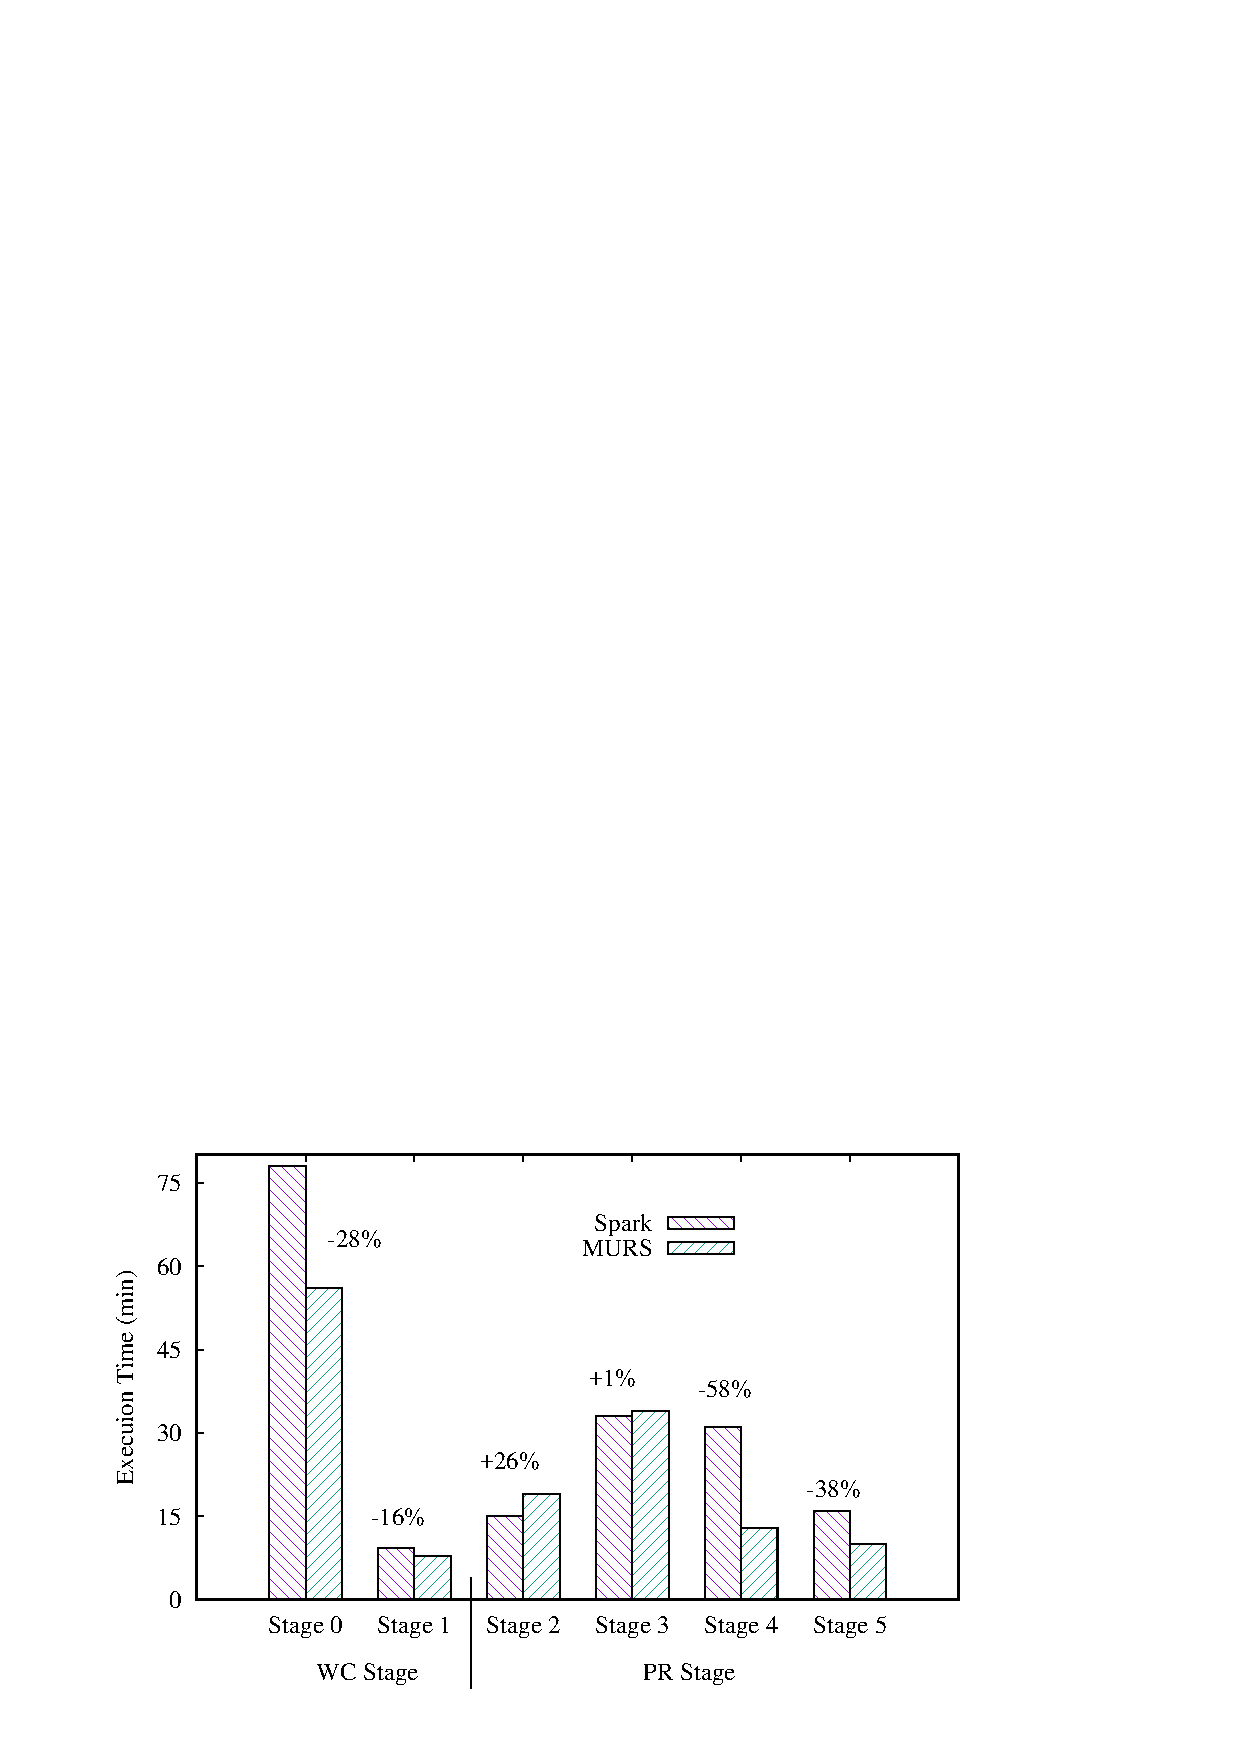
\includegraphics[width=0.4\textwidth]{multitalent-exec.pdf}
%\vspace{-2mm}
\caption{The Execution Time of PR Job and WC Job}
%\vspace{-4mm}
\label{fig:pr-wc-exec}
\end{figure}

\begin{figure}[!t]
\centering
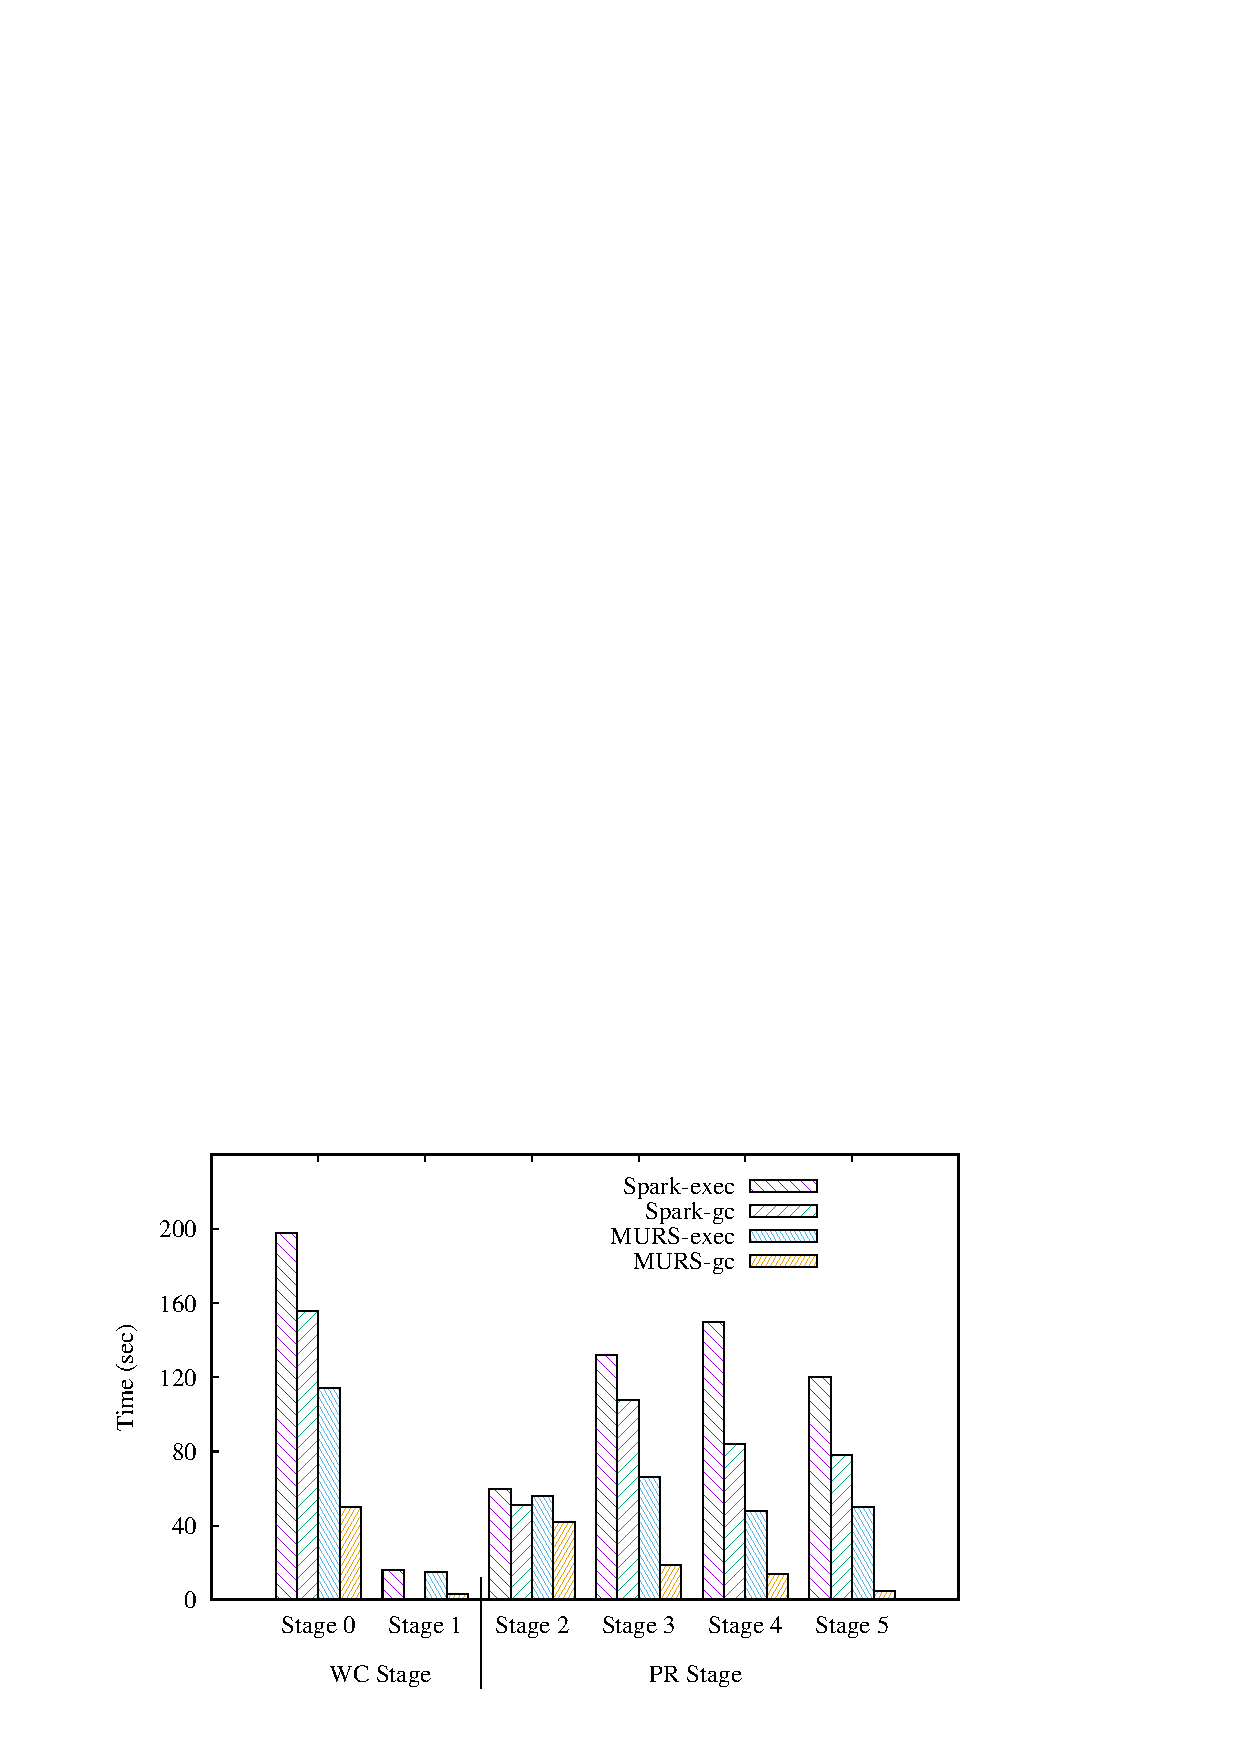
\includegraphics[width=0.4\textwidth]{pr-wc-gc.pdf}
%\vspace{-2mm}
\caption{The Execution and GC Time of Tasks in PR and WC}
%\vspace{-4mm}
\label{fig:pr-wc-gc}
\end{figure}

Before WC completes, tasks in PR and WC both result in memory pressure. However, tasks in PR belong to linear model, while tasks in WC belong to sub-linear model. MURS will suspend these tasks in PR to prevent heavy memory pressure, thus tasks in WC can have a lower execution time.

The execution time of the second stage of PR increases because tasks in PR are always classified to heavy tasks in this scene. In the second stage, PR caches all intermediate data in memory until the job completes. Then the memory manager requires many CPU cycles to trace the caching data objects; and less memory space is accessible for execution, which results in heavy garbage collection. While MURS intends to mitigate the heavy memory pressure, tasks in PR are always classified to heavy tasks because there are no other tasks belong to linear models. Thus, the waiting time of suspended tasks increases greatly although the garbage collection time decreases in Figure~\ref{fig:pr-wc-gc}, and the second stage in PR is even worse in MURS than in Spark for service. Fortunately, as WC completes early, subsequent stages  in MURS suffer much less memory pressure (the garbage collection can be decreased as much as 94\% in some tasks in Figure~\ref{fig:pr-wc-gc}), and performance improves more. 

\subsection{Avoidance of spill}

MURS sets the red value to avoid spill when memory pressure is heavy in these systems who provide spill. We take the evaluation in the last section, which runs PR and WC in the Spark for service, to measure the spill tasks. MURS estimates the size of required memory space for each task, and ensures that running tasks can complete with the remaining memory space. As the estimation is inaccurate to some extent, we find that fewer tasks will still spill in MURS, as shown in Table~\ref{table:spill}. There are no spill tasks in WC in MURS and the spill tasks in PR decreased from 32\% to 2.5\% in comparing to Spark.

\begin{table}[!t]
\small
\centering
\caption{Spill Tasks in MURS and Spark}
\begin{tabular}{| c | c | c | c | c | c | c | c |}

\hline
\multirow{2}{*}{} & \multirow{2}{*}{\textbf{App}} & \multicolumn{3}{| c |}{\textbf{Spill Percentage}} & \multicolumn{3}{| c |}{\textbf{Spill Size (MB)}} \\
\cline{3-8}
 & & total & spill & percent & min & mid & max \\
\hline
\multirow{2}{*}{Spark} & WC & 1000 & 91 & 9\% & 0 & 0 & 710 \\
\cline{2-8}
 & PR & 1500 & 480 & 32\% & 310 & 367 & 439 \\
\hline
\multirow{2}{*}{MURS} & WC & 1000 & 0 & 0\% & - & - & -  \\
\cline{2-8}
 & PR & 1500 & 37 & 2.5\% & 0 & 0 & 458 \\
\hline

\hline
\end{tabular}
%\vspace{-2mm}
 
%\vspace{-6mm}
\label{table:spill}
\end{table}

We should acknowledge that error exists in the avoidance of spill. The sampler in MURS counts two important metrics of one task: the percentage of processed records in total records, and the current allocated memory space for this task. We can quickly get the required memory space based on these two metrics. When memory pressure reaches the red value, we suspend parts of tasks and leave enough remaining memory space for running tasks. As the estimate is based on sampling, error exists in the estimated size of allocated memory space, especially when the value in some key-value pairs is a collection. Different records have different sizes because the number of values inside a collection is different, such as \textit{groupByKey} in PR. Some hot keys may result in substantial error. Thus, it can be accepted that there are even fewer spill tasks in MURS.

\subsection{Memory pressure in multi-launch}

Some systems for service are oversold and launches multiple tasks than the original configuration. When the service is idle, it has efficient memory usage. However, if the service comes to busy, the memory pressure is uncontrollable and the performance will degrade quickly when memory pressure is heavy. MURS is appropriate for this problem as it keeps the advantage in light memory pressure but prevents memory pressure increasing fast in heavy memory pressure. We choose WC here and two datasets to compare the impact of multi-launch MURS with Spark. We submit WC independently here to clearly distinguish the light and heavy memory pressure, and MURS can also work as mentioned in Section~\ref{sec:desgin}. WC processes data as (\textit{K}, \textit{V}), while \textit{K} means the words in the dataset. Thus, the number of words will decide the size of shuffle buffer, and more words will result in more memory pressure. As shown in Figure~\ref{fig:subfig:wc-million}, the GC time can be increased to 31.8\%, but the reduction of execution time is 11.6\% when the number of words is 1 million; the reduction of execution time is 22.9\% and the GC time can be 45.2\% when the number of words increases to 100 million in Figure~\ref{fig:subfig:wc-billion}.

%Although MURS is designed for data processing systems for service, we find it can also work well in batch processing when all running tasks have the same model. We choose WC here and two datasets to compare the impact of multi-launch in different memory pressures. WC process data as (\textit{K}, \textit{V}), while \textit{K} means the words in the dataset. Thus, the number of words will decide the size of shuffle buffer, and more words will result in more memory pressure. As shown in Figure~\ref{fig:subfig:wc-million}, the GC time can be increased to 31.8\%, but the reduction of execution time is 11.6\% when the number of words is 1 million; the reduction of execution time is 22.9\% and the GC time can be 45.2\% when the number of words increases to 1 billion in Figure~\ref{fig:subfig:wc-billion}.

\begin{figure}[!t]
\centering
\subfigure[Light memmory pressure]{
\label{fig:subfig:wc-million}
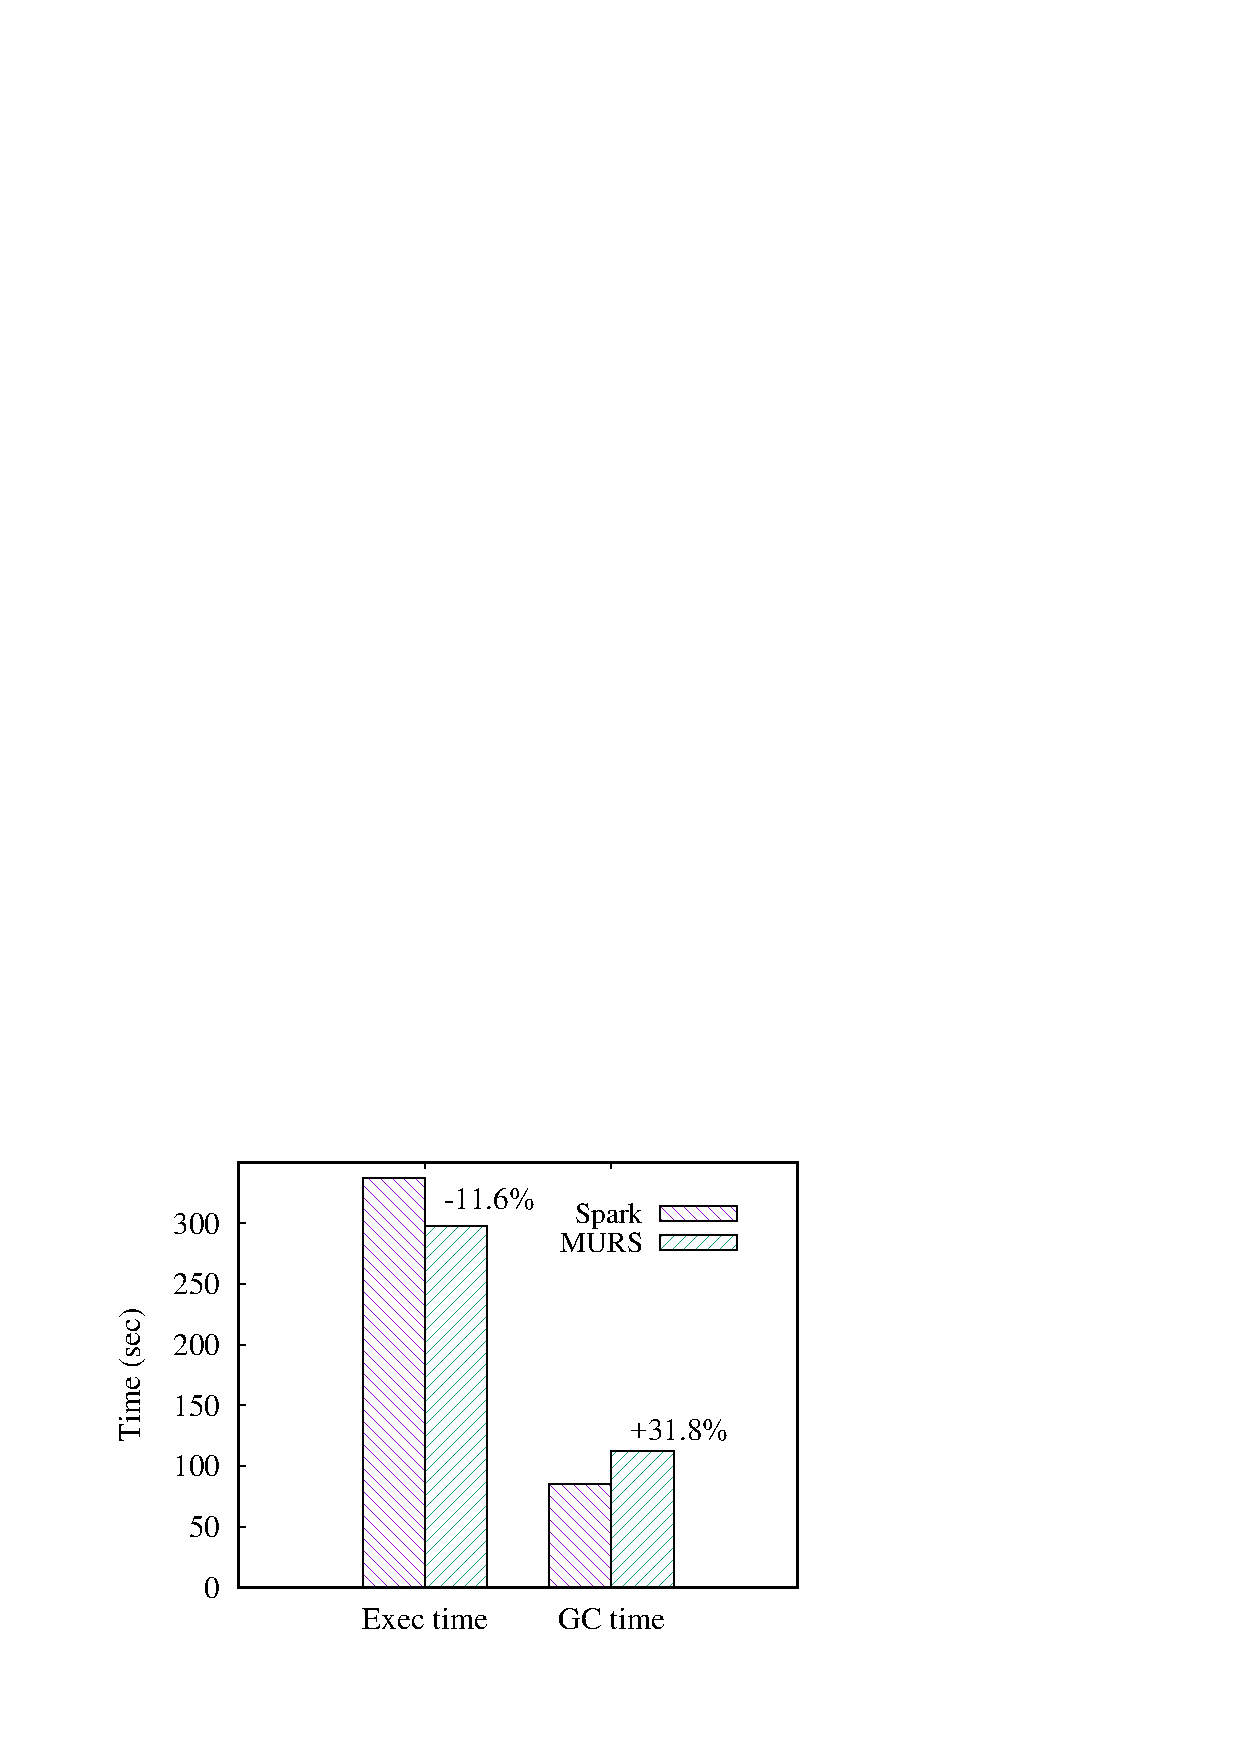
\includegraphics[width=0.231\textwidth]{wc-million.pdf}}
\hspace{-1.3ex}
\subfigure[Heavy memory pressure]{
\label{fig:subfig:wc-billion}
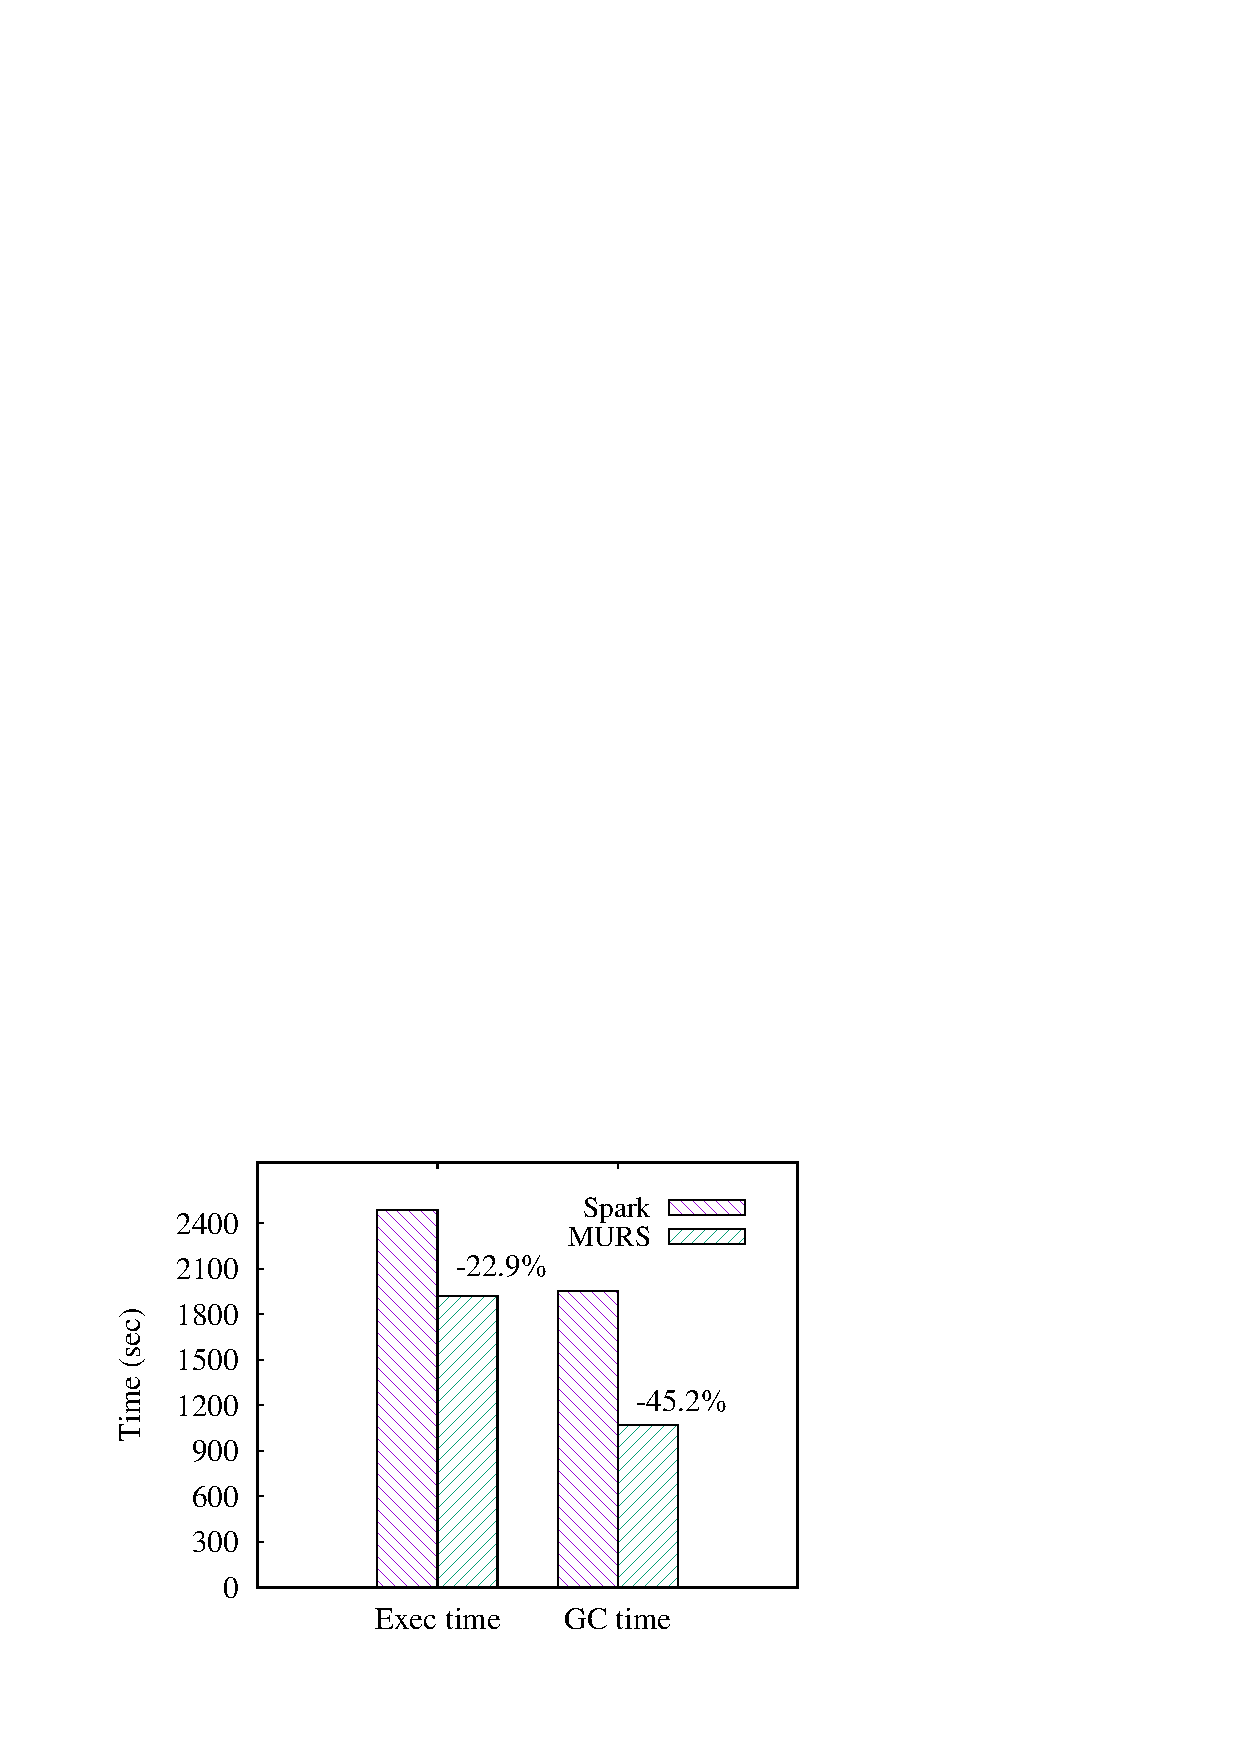
\includegraphics[width=0.231\textwidth]{wc-billion.pdf}}
\label{fig:wc-result}
%\vspace{-2mm}
\caption{Multi-launch with MURS when service is busy}
%\vspace{-4mm}
\end{figure}

Light memory pressure usually means that memory space will suffer less allocation and reclamation. Multi-launch increases the parallelism as well as the memory pressure, which properly increase the frequency of memory allocation and reclamation. This improves the efficiency of memory usage. Thus the services work well with multi-launch in Figure~\ref{fig:subfig:wc-million}. MURS remains the advantages in this scene. However, when the words increases to 100 million, memory pressure is high and the throughout is only 25.6\%. Frequent garbage collection degrades the performance quickly. MURS will suspend numbers of tasks to prevent the increase of memory pressure, thus both execution time and garbage collection time decrease in Figure~\ref{fig:subfig:wc-billion}.



















%%%%\begin{comment}

\subsection{Batch Processing}

\subsubsection{Impcat of Shuffle Function}
WordCount in Spark benchmark is an original MapReduce application. WC has two stages: the first stage reads data from HDFS and writes shuffle buffers; the second stage reads data from shuffle buffers and then function \textit{reduceByKey} is used to get the result. Shuffle buffers process data as (\textit{Key},\textit{Value}) while \textit{Key} means the words in dataset. Thus the number of words will decide the size of shuffle buffers, and more words will result in more memory pressure. As shown in Figure~\ref{fig:subfig:wc-million}, the GC time can be increased to 31.8\% but the reduction of execution time is 11.6\% when the number of words is 1 million; the reduction of execution time is 22.9\% and the GC time can be 45.2\% when the number of words increases to 1 billion in Figure~\ref{fig:subfig:wc-billion}.

When the size of words is small, the shuffle buffers will have less keys. The size of shuffle buffers will not result in heavy memory pressure which can also be proved by the light garbage collection. MURS provides multi launch to increase the memory pressure and parallelism of job, the running tasks is 1.5x than Spark. Thus the execution time decreases but the garbage collection time increases in Figure~\ref{fig:subfig:wc-million}. However, when the words increases to 1 billion, memory pressure can be high and the throughout is only 25.6\%. MURS will stop numbers of tasks to prevent the increase of memory pressure and both execution time and garbage collection time will decrease in Figure~\ref{fig:subfig:wc-billion}. 

\subsubsection{Impcat of Caching and Shuffle Function}
PageRank(PR) will firstly cache important intermediate data of function \textit{groupByKey} in memory. Each of the appending several iterations is a stage in the job. The main functions in each stage are \textit{join} and \textit{reduceByKey}. The function \textit{join} not belongs to shuffle function in PR. We test 10 iterations here and the result is shown in Figure~\ref{fig:pr-stagetime}. While the first stage just read data from HDFS, the memory pressure is light. After stages will suffer from caching data in memory. The size of caching data in each node is 4.1GB-5.3GB. Different stage has different memory pressure, the max execution time has the speed up of 2.1x to the min in Spark. Different memory pressure and tasks result in different performance of MURS. The best reduction of execution time can be 56\% and the average reduction is 44\% for computing stages.

\begin{figure}[!t]
\centering
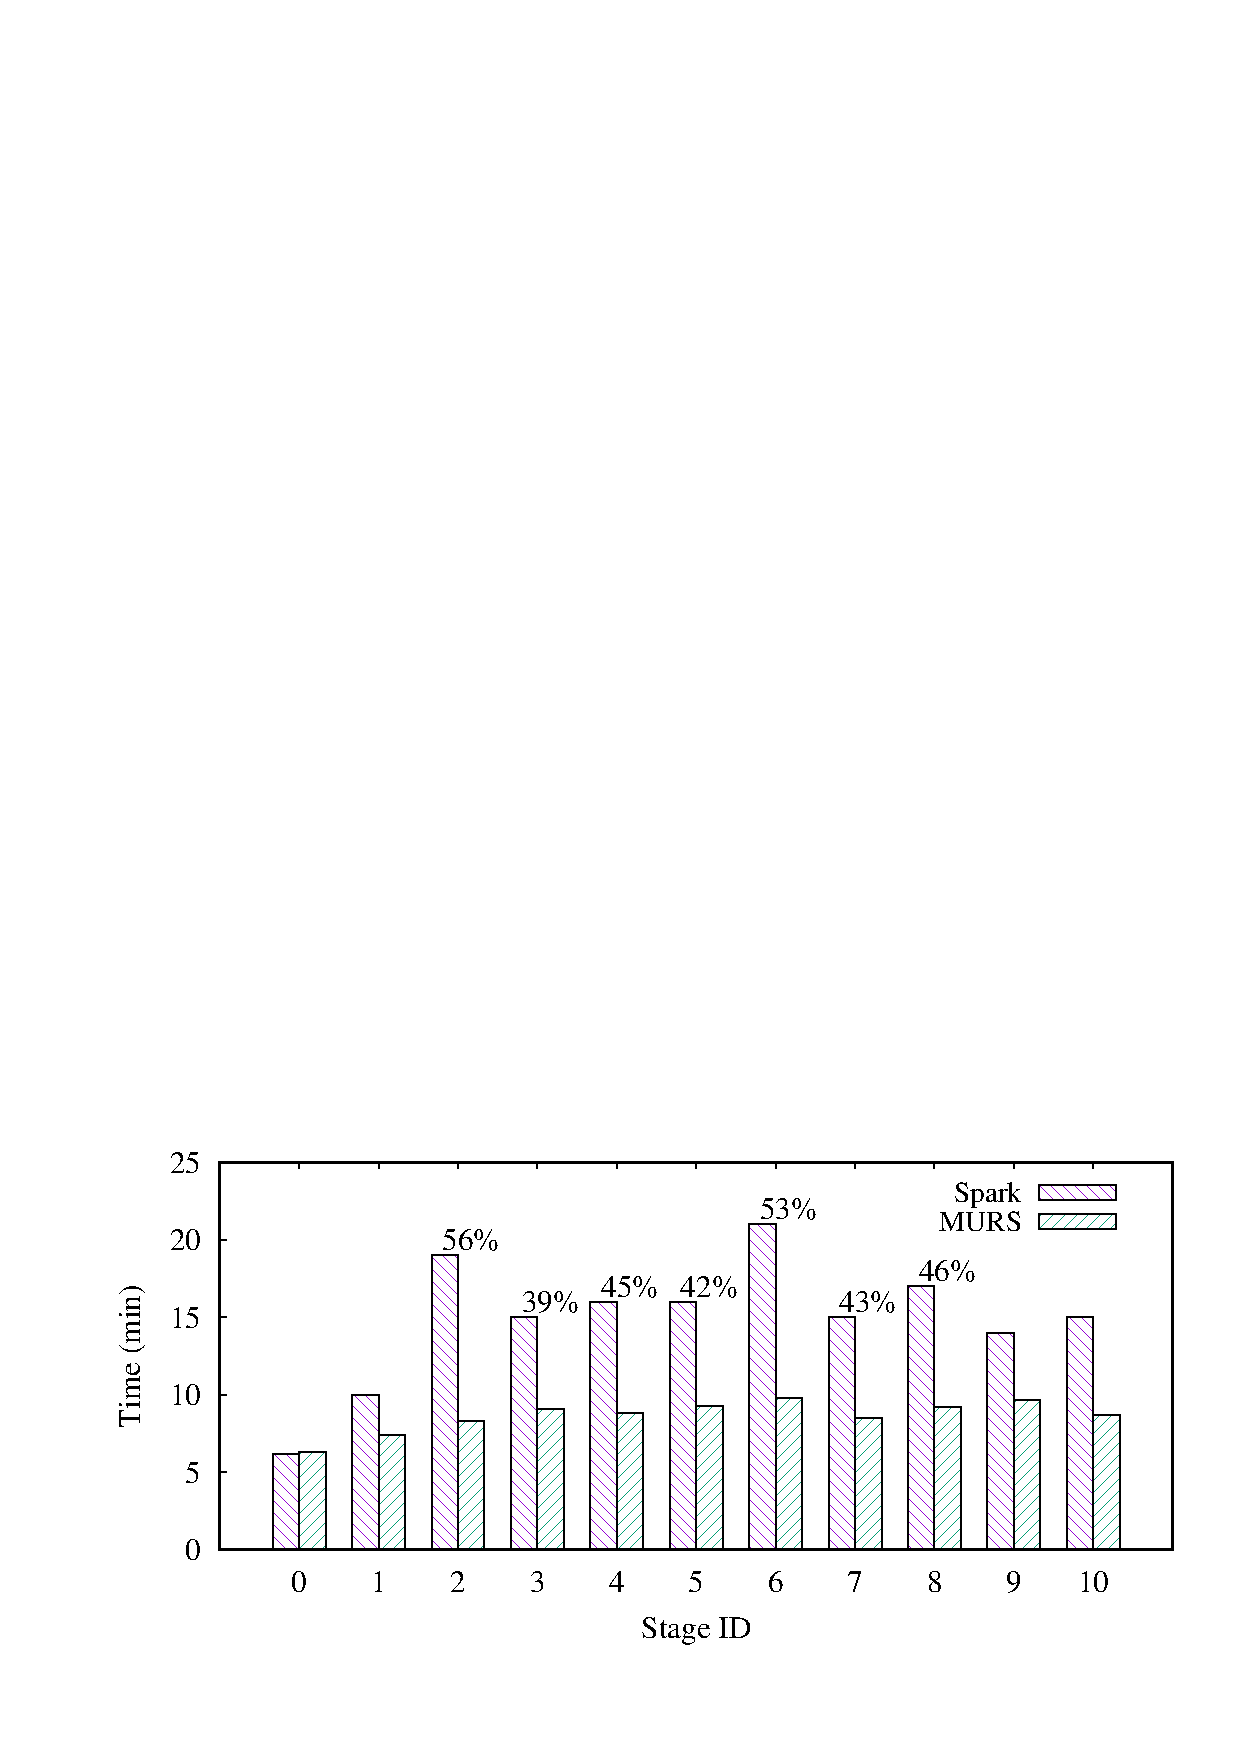
\includegraphics[width=0.45\textwidth]{pr-stagetime.pdf}
\vspace{-2mm}
\caption{The Result of Each Stages in PageRank}
\vspace{-2mm}
\label{fig:pr-stagetime}
\end{figure}

The caching data cost constant memory space because the caching data has same lifetime in the job. While less execution memory space is accessible for shuffle operation, the same data objects will result in worse memory pressure and more frequently garbage collection. The improvement of PageRank in MURS is benefit from three points: GC reduction, spill avoidance  and stopping tasks.

\begin{figure}[!t]
\centering
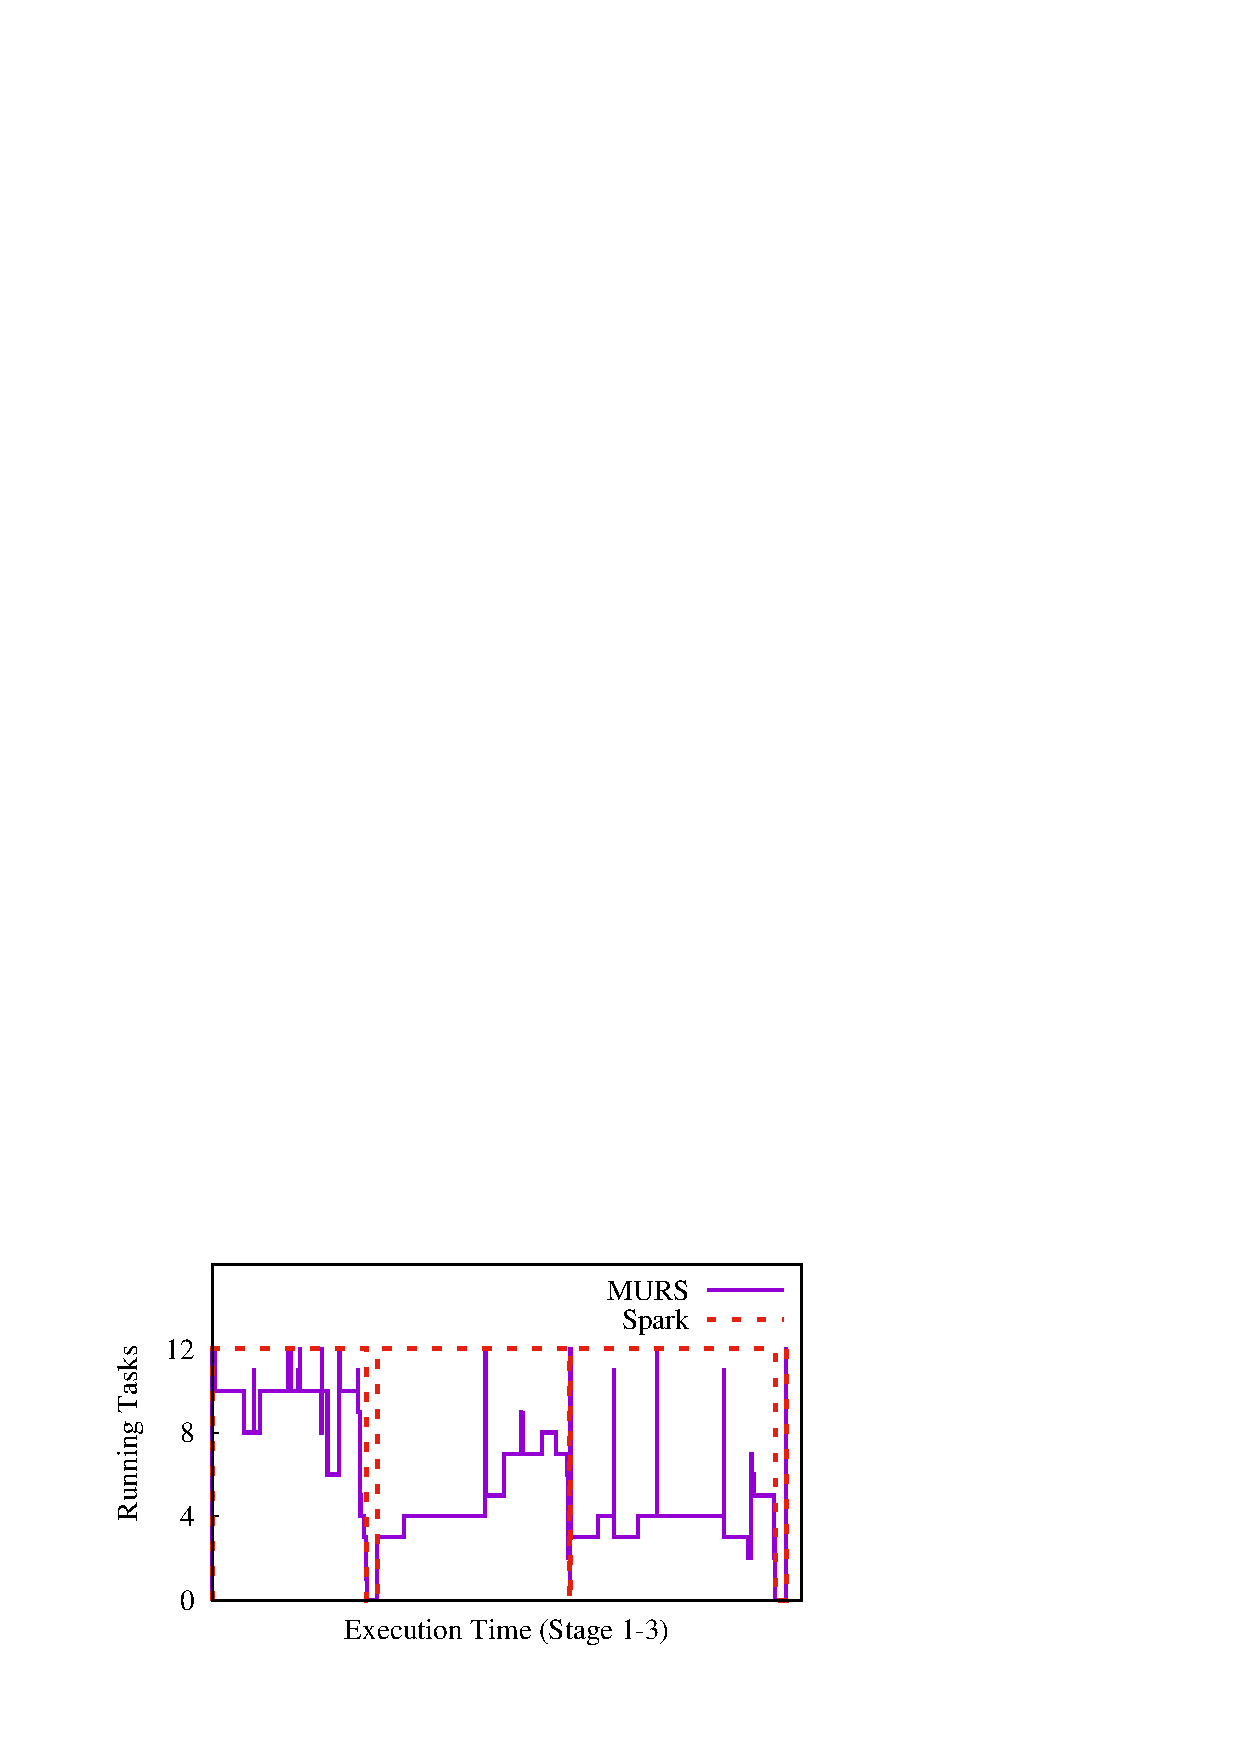
\includegraphics[width=0.35\textwidth]{pr-runtasks.pdf}
\vspace{-2mm}
\caption{The Number of Running Tasks in MURS}
\vspace{-2mm}
\label{fig:pr-runtasks}
\end{figure}

\textbf{Stopping tasks} The core scheduling in MURS is stopping parts of tasks to prevent heavy memory pressure, thus we firstly analysis the count of running tasks as shown in Figure~\ref{fig:pr-runtasks}. The first stage has no caching data but some shuffle buffers in memory. The shuffle buffer will be live in JVM heap until write to disk, thus they result in some memory pressure and our scheduler stop two tasks accordingly. When the job runs in after stages, caching data will stay in memory until the job complete. The heavy memory pressure result in more stopped tasks.

\begin{figure}[!t]
\centering
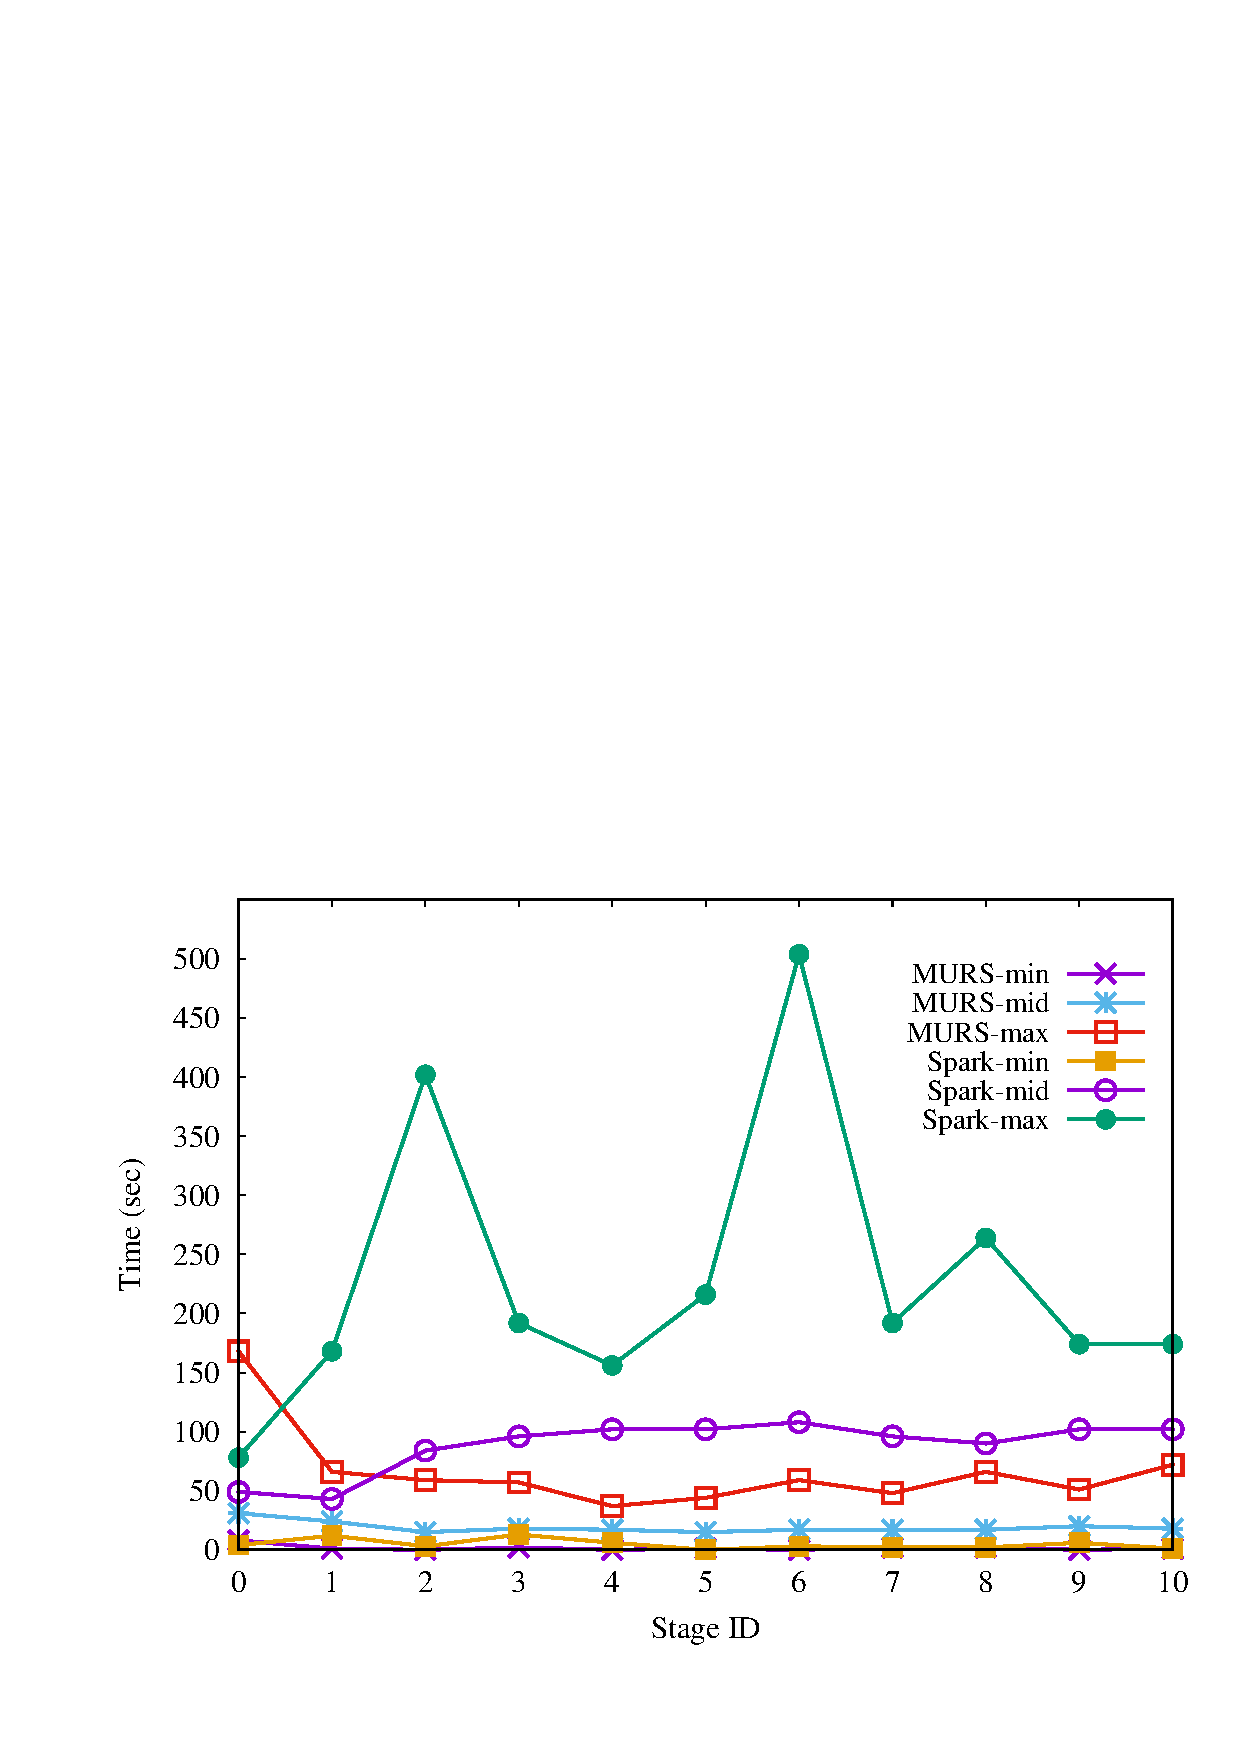
\includegraphics[width=0.45\textwidth]{pr-gc.pdf}
\vspace{-2mm}
\caption{The GC of Total Tasks in PageRank}
\vspace{-4mm}
\label{fig:pr-gc}
\end{figure}

\textbf{GC reduction} Each task suffers from different garbage collection, as shown in Figure~\ref{fig:pr-gc}. We compare the minimum, median and maximum of total tasks. Each guideline in MURS is better than Spark. The median of garbage collection time in MURS has the speed up of 5.5x. The reduction of garbage collection can be more cleared with the peak execution memory of each task. Peak execution memory of each task is 457MB/533MB/868MB(min/mid/max) in MURS, and 369MB/493MB/597MB(min/mid/max) in Spark. As MURS stop some tasks to avoid the cost of memory space which will be occupied for a long time, other running tasks has more execution memory. While the same memory space is provided for less running tasks, the peak execution memory of each tasks will be high. If the peak execution memory is high, tasks can run without heavy memory pressure because less garbage collection will occur. After the running tasks release their occupied space, stopped tasks can also improve their peak execution memory. Thus the memory pressure in MURS is lighter than Spark, and more execution memory slow down the heavy garbage collection essentially.

We can also get the conclusion that the straggler can be avoided in some way. The max garbage collection time and the average time is much near in MURS but fluctuating serious in Spark. As the time of garbage collection makes up the important part of execution time, tasks with long period of garbage collection will have long execution time. If the execution time of one task exceeds the average time of completed tasks, we regard it as an straggler. Thus MURS will have low probability to produce the straggler.

\begin{table}[!t]
\small
\centering
\begin{tabular}{| c | c | c | c | c | c | c | c |}

\hline
\multirow{2}{*}{} & \multirow{2}{*}{Stage} & \multicolumn{3}{| c |}{Spill Percent} & \multicolumn{3}{| c |}{Spill Size (MB)} \\
\cline{3-8}
 & & total & spill & percent & min & mid & max \\
\hline
\multirow{2}{*}{Spark} & stage6 & 300 & 185 & 62\% & 0 & 370 & 480 \\
\cline{2-8}
 & stage1 & 300 & 52 & 17\% & 0 & 0 & 471 \\
\hline
\multirow{2}{*}{MURS} & stage6 & 300 & 0 & 0\% & - & - & -  \\
\cline{2-8}
 & stage1 & 300 & 1 & 1\% & 0 & 0 & 399 \\
\hline

\hline
\end{tabular}
\vspace{-2mm}
\caption{Spill Tasks in MURS and Spark} 
\vspace{-4mm}
\label{table:pr-spill}
\end{table}

\textbf{Spill avoidance} Spark has several spill tasks in each stage, and only one stage of MURS has spill tasks, as shown in Table~\ref{table:pr-spill}. No matter in the first stage or other stages, most tasks can avoid spilling in MURS although they would spill in Spark. The fundamental reason is also more execution memory. MURS has the spill computing algorithm to avoid spilling. After stopping tasks, remain space are enough to running tasks is just the goal of MURS. While multi launch is available, the spill computing algorithm is more functional to control the running tasks. We notice that spill also appear in MURS, there are two points here: 1) estimating the remaining using space of one running task is not usually accurate; 2) the available memory space of one thread in JVM is limited (1/2N at least and 1/N at most while N is the number of running threads in JVM). Spill can result in expensive disk IO, thus the performance can be better.% in MURS.

\subsection{Multi-tenant}

Spark JobServer can provide multi-tenant for Spark. We submit both WordCount and PageRank to the Spark JobServer to test the performance of MURS in multi-tenant. We set the number of iterations to be 3 in PageRank, when the WordCount completes, PageRank usually complete the second stage. The result is shown in Figure~\ref{fig:mul-exec}. The execution time of WordCount decreased 28\% but at the same time the execution time of PageRank increased 26\%. After WordCount is complete, the execution of PageRank can be decreased to 58\%. We should notice that, when the WordCount is complete the PageRank runs both in Stage 2.

In the first stage, tasks in PR and WC are both \textit{ShuffleMapTask} which result in memory pressure through the shuffle buffer in shuffle writer. However, the function APIs in PR is \textit{groupBykey} which is a non-aggregation, it increases the size of shuffle buffer for each processed record. The function APIs in WC is \textit{reduceByKey} which is an aggregation, it increases the size of shuffle buffer only when the \textit{K} of processed record has never appeared. Obviously, the tasks in PR belong to linear while the tasks in WC belong to sub-linear. Our scheduler will stop the tasks of PR to prevent the heavy memory pressure, thus the tasks of WC can have less execution time. The pity is that the waiting time of stopped tasks increased much. Fortunately, as WC completes early, the third stage (Stage 2) in MURS suffer much less memory pressure, and the performance improves more. This is much important in multi-tenant, not only the tasks with heavy influence on memory pressure can execute more quickly, but also these tasks with light influence can avoid the memory pressure. The service of all tenant, which means PR and WC, can be better.

\end{comment}


